%% ----------------------------------------------------------------
%% shortened_main.tex -- Shortened version of the project report for
%% Turnitin plagiarism checking. Contains the introduction through the
%% conclusion only. No title page, abstract, statement of originality,
%% acknowledgements, table of contents, bibliography, or appendices.
%% ----------------------------------------------------------------
\documentclass[oneside]{ecsproject}
\graphicspath{{./}{figures/}{../Figures/}}
\usepackage[numbers,sort&compress]{natbib}
\usepackage{booktabs}
\usepackage{amsmath}
\usepackage{amssymb}
\usepackage{microtype}
\usepackage{xcolor}
\usepackage{listings}
\usepackage{placeins}
\usepackage{pdfpages}
\usepackage{tikz}
\usepackage{pgfplots}
\pgfplotsset{compat=1.18}
\usetikzlibrary{matrix,positioning,arrows.meta,fit,shapes.geometric,calc,decorations.pathreplacing}
\hypersetup{colorlinks=true}
\input{Definitions}

\newcommand{\setbodymargins}{
\setmarginsrb           {1.2in}
                        {0.6in}
                        {0.8in}
                        {0.8in}
                        {20pt}
                        {0.25in}
                        {9pt}
                        {0.3in}
}

% Suppress "undefined reference" warnings from labels that live only in the
% removed appendices or bibliography; these show as ?? in the output but do
% not affect the prose the plagiarism check is looking at.
\begin{document}
\setbodymargins
\pagenumbering{arabic}
\setcounter{page}{1}

% !TEX root = ../main.tex
\chapter{Introduction}
\label{ch:introduction}

\section{Motivation}

Sparse matrix--dense matrix multiplication (SpMM) is one of the fundamental
computational kernels in modern machine learning and graph-based computing.
In graph neural networks (GNNs) it embodies the neighbourhood aggregation
step, in which a sparse adjacency matrix is multiplied against a dense
feature matrix~\citep{graphsage2017, gat2018}. In large-scale recommender
systems, collaborative filtering relies on sparse user--item interaction
matrices whose dimensions can reach hundreds of millions of
rows~\citep{covington2016youtube}. In scientific simulation, it is the
inner loop of iterative solvers for finite-element and finite-difference
discretisations. The same pattern appears in transformer attention with
sparse masks and in the weight-matrix multiply step of pruned and
compressed neural networks~\citep{han2016eie}. Across all of these
workloads the common denominator is that the useful arithmetic is only
a small fraction of the work that a general-purpose processor actually
performs, with most cycles spent chasing indirect indices, handling row
boundaries, and issuing scattered memory accesses.

With the rapid rise in demand for AI, there has been a matching rise in
demand for better model algorithms, more data, and above all more computation.
On the compute side, most AI workloads are now executed on
application-specific integrated circuits (ASICs), since these have been shown to
maximise throughput, energy efficiency, and cost-effectiveness for the
particular matrix operations that AI models need to run. Some of the most
well-known commercial examples are the Tensor Processing Unit (TPU) from
Google and the Neural Processing Unit (NPU) from Apple. The design of any
such ASIC, however, almost always begins with prototyping on a Field
Programmable Gate Array (FPGA), because FPGAs can execute many operations
in parallel and are easily reconfigurable, which keeps architectural
exploration inexpensive and quick. An
FPGA-hosted accelerator for SpMM is therefore a natural first step towards
a fully custom silicon implementation, and is the platform targeted by
this project.

\section{Project Aim}

The aim of this project is to design, implement, and evaluate a
RISC-V-compatible hardware accelerator for compressed sparse row (CSR) SpMM on
the Terasic DE1-SoC FPGA board. The accelerator must integrate cleanly
into a small system-on-chip (SoC), share on-chip block RAM with the CPU,
and deliver a measurable, reproducible speedup over a comparable software
implementation while remaining understandable at the register-transfer
level (RTL) and transparent in its benchmarking methodology. A secondary
aim is to isolate the individual contribution of each optimisation step,
so that the dominant performance bottleneck can be identified through
direct measurement rather than assumption. To achieve this, the design
is developed in three stages (a baseline accelerator, a parallel
DSP-oriented multiply-accumulate enhancement, and a symmetric INT8
packing stage), forming a controlled experimental path in which only
one design dimension is changed at a time.

Beyond the core aim, the project defined three stretch goals at the
outset. The first was to introduce a custom RISC-V instruction to trigger
the accelerator directly from the CPU pipeline, rather than through a
memory-mapped register write, which would reduce launch overhead and
demonstrate that the PicoRV32 soft core can be extended at the instruction
set level. The second was to implement runtime INT8 quantisation so that
operand fetch bandwidth could be reduced by packing four quantised values
into a single 32-bit RAM word. The third was to extend the accelerator
with optional activation functions and a max-pooling stage, so that it
could serve as a building block for a small inference pipeline rather
than as a standalone kernel. Of the three, the INT8 quantisation goal
was achieved and is reported in full in this work; the remaining two
are discussed as future work in Chapter~\ref{ch:conclusion}.

\section{Report Structure}

The remainder of this report is structured as follows.
Chapter~\ref{ch:motivation} reviews the background needed to justify the
design choices, covering SpMM workloads, sparse data formats, prior
accelerator work and the rationale for FPGAs.
Chapter~\ref{ch:platform} defines the implemented SoC platform and its
memory-mapped I/O interface. Chapter~\ref{ch:design} presents the
accelerator architecture and each optimisation step in detail.
Chapter~\ref{ch:methodology} defines the hardware verification approach
and the unit and integration testbenches used to check the RTL.
Chapter~\ref{ch:firmware} describes the bare-metal firmware, the
benchmark suite, and the measured cycle-count and correctness results
across the three optimisation stages. Chapter~\ref{ch:reflection}
discusses lessons learned and project management, and
Chapter~\ref{ch:conclusion} closes the report with a summary and proposed
future work.

\chapter{Background and Literature Review}
\label{ch:motivation}

There is a vast body of algorithms for Sparse Matrix Multiplication (SpMM),
as well as many different storage formats for converting sparse matrices into
representations that can be operated on efficiently. This chapter provides
the information needed to understand the context and design decisions taken
throughout this project, alongside the goals that were set out at the start.
If any of the material that follows is unfamiliar, a more elementary
overview of SpMM and the CSR format is given in
Appendix~\ref{app:spmm-background}, and further reading can be pursued
through the references cited in each section.
\section{SpMM in Modern Workloads}

The motivation for a dedicated SpMM accelerator is made concrete by the
sparsity levels that real workloads exhibit. Figure~\ref{fig:sparsity-levels}
summarises representative density ranges across four workload classes: in
each case, the fraction of nonzero entries is small enough that storing and
operating on the matrix in dense form would be wasteful by one to five
orders of magnitude.

\begin{figure}[htbp]
  \centering
  \hspace*{-1.5cm}%
  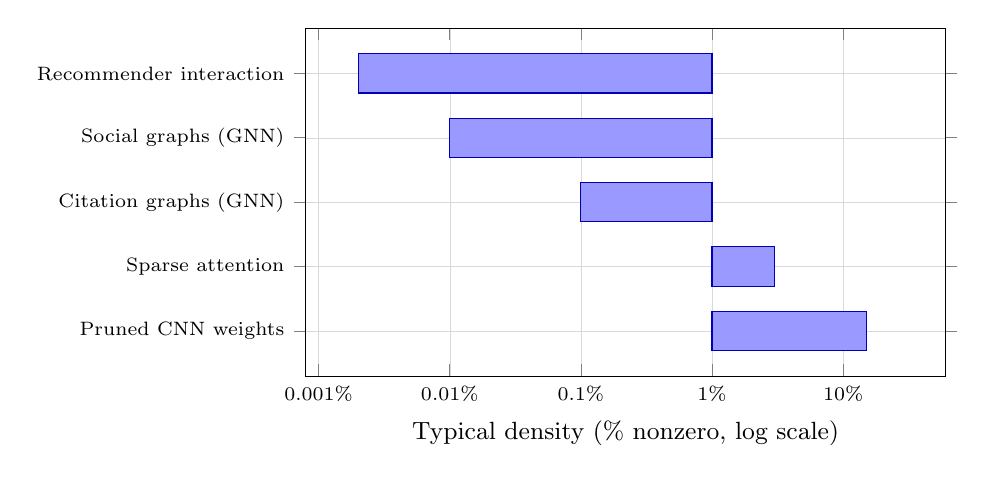
\begin{tikzpicture}
    \begin{axis}[
      width=0.8\linewidth, height=6cm,
      xbar,
      xmode=log,
      log basis x=10,
      xmin=0.0008, xmax=60,
      xlabel={Typical density (\% nonzero, log scale)},
      ytick={1,2,3,4,5},
      yticklabels={
        {Recommender interaction},
        {Social graphs (GNN)},
        {Citation graphs (GNN)},
        {Sparse attention},
        {Pruned CNN weights}},
      y dir=reverse,
      ymin=0.3, ymax=5.7,
      bar width=5mm,
      xtick={0.001,0.01,0.1,1,10},
      xticklabels={0.001\%,0.01\%,0.1\%,1\%,10\%},
      tick label style={font=\scriptsize},
      label style={font=\small},
      grid=major,
      major grid style={line width=.1pt, draw=gray!30},
    ]
      \addplot[fill=blue!40, draw=blue!70!black] coordinates {
        (0.002, 1)
        (0.01,  2)
        (0.1,   3)
        (3,     4)
        (15,    5)
      };
    \end{axis}
  \end{tikzpicture}
  \caption{Representative density ranges for matrices encountered in four
           classes of modern workload. Social and citation graphs in GNN
           benchmarks such as \texttt{ogbn-arxiv} and \texttt{Reddit} typically
           have densities below 0.1\%~\citep{graphsage2017}; large-scale
           recommender interaction matrices are often two orders of magnitude
           sparser still~\citep{covington2016youtube}. Pruned CNNs sit at the
           other end of the range, retaining 10--20\% of their weights after
           aggressive pruning~\citep{han2016eie}. In every case, an SpMM
           execution model that iterates only over the nonzeros avoids between
           90\% and $>99.99$\% of the arithmetic that a dense multiply would
           perform.}
  \label{fig:sparsity-levels}
\end{figure}

\subsection{Graph Neural Networks}

Graph neural networks (GNNs) represent the most rapidly growing class of workloads
in which SpMM appears as a first-class primitive. In message-passing GNNs such as
GraphSAGE~\citep{graphsage2017} and Graph Attention Networks~\citep{gat2018}, each
layer computes
\[
  H^{(l+1)} = \sigma\!\left( \hat{A} \, H^{(l)} \, W^{(l)} \right),
\]
where $\hat{A}$ is the normalised sparse adjacency matrix of the input graph,
$H^{(l)}$ is the dense feature matrix at layer $l$, and $W^{(l)}$ is a dense
weight matrix. The product $\hat{A} \, H^{(l)}$ is a sparse--dense matrix
multiply: $\hat{A}$ is sparse (real-world social and citation graphs can have
densities below 0.01\%), while $H^{(l)}$ is dense with feature dimension
typically 64--2048. This SpMM step dominates GNN inference time in practice,
particularly for large graph datasets where $\hat{A}$ has billions of edges.

\subsection{Recommender Systems and Sparse Embedding Lookup}

Industrial recommender systems such as the YouTube recommendation engine
\citep{covington2016youtube} maintain item--feature embedding tables that can
reach hundreds of millions of rows. The forward pass performs sparse embedding
lookups that reduce to a row-gather SpMM on the interaction matrix. Because the
interaction patterns are highly sparse and the embedding matrices are dense, the
memory-access pattern is irregular and the workload is inherently SpMM-shaped.

\subsection{Scientific Computing}

In finite-element and finite-difference simulation, sparse matrices arise from
the discretisation of differential operators on computational meshes. The
structure of the sparse factor is dictated by the mesh topology, which is
problem-dependent and generally irregular. SpMM in this setting appears in
multivector iterative solvers such as block GMRES and Lanczos methods, where
each Krylov iteration applies the sparse system matrix to a block of several
dense vectors simultaneously.

\subsection{Compressed and Pruned Neural Networks}

Weight pruning removes less-significant connections from a dense neural network,
increasing the proportion of zero weights and making weight matrices suitable for
sparse representation. Han et al.~\citep{han2016eie} demonstrated that networks
pruned to 80--90\% sparsity can be represented and executed in compressed form
with significant reductions in energy and storage. When combined with INT8
quantisation, as in the EIE design, SpMM on the compressed weight matrix becomes
the dominant kernel. The same principle applies to attention heads in transformers
that adopt sparse attention patterns.

\section{Why Sparsity Changes the Design Problem}

\subsection{The FLOP-to-Bandwidth Mismatch}

Dense matrix multiplication exhibits high operational intensity: for an
$M \times K \times N$ dense GEMM, the ratio of FLOPs to bytes loaded is
$O(N)$ when data is reused across the $N$ output columns. Sparse matrix
multiplication loses this reuse structure. For a CSR SpMM with $\text{NNZ}$
nonzeros, the number of useful MACs per byte of CSR index data fetched is
\[
  \text{OI} = \frac{2 \cdot \text{NNZ} \cdot N}
                   {\text{NNZ} \cdot (4 + 4) + (M + 1) \cdot 4 + \text{NNZ} \cdot 4 \cdot N},
\]
where the denominator accounts for \texttt{colidx} (4 bytes per entry),
\texttt{values} (4 bytes per entry), \texttt{rowptr} (4 bytes per pointer), and
the dense $B$ segment reads (4 bytes per column per nonzero). For small $N$ and
low density, the operational intensity is significantly below the roofline knee
of typical on-chip BRAM systems~\citep{williams2009roofline}, confirming that
SpMM is memory-bandwidth-limited rather than compute-limited on most platforms.

\subsection{Irregular Access and Control-Flow Overhead}

Beyond raw bandwidth, SpMM imposes control overhead that dense accelerators are
not designed to handle. For each nonzero $a_{ij}$, the hardware must:
\begin{enumerate}
  \item read the column index $j$ from \texttt{colidx};
  \item compute the address of the relevant row of $B$ as $\text{B\_base} + j \cdot N$;
  \item read the $N$ values of $B[j, :]$; and
  \item accumulate $a_{ij} \cdot B[j, n]$ into $C[i, n]$ for each column $n$.
\end{enumerate}
Steps (1) and (2) involve indirection: the address of the $B$ row is not known
until the column index has been loaded. This pointer-chasing pattern breaks
prefetching and creates a data-dependent dependency chain that is difficult for
out-of-order processors to hide. On a simple in-order core such as PicoRV32,
each nonzero must be handled sequentially, making the control overhead dominate
the total execution time. Figure~\ref{fig:access-pattern} contrasts the
predictable stride of a dense traversal with the indirect, data-dependent
address sequence that CSR SpMM produces.

\begin{figure}[htbp]
  \centering
  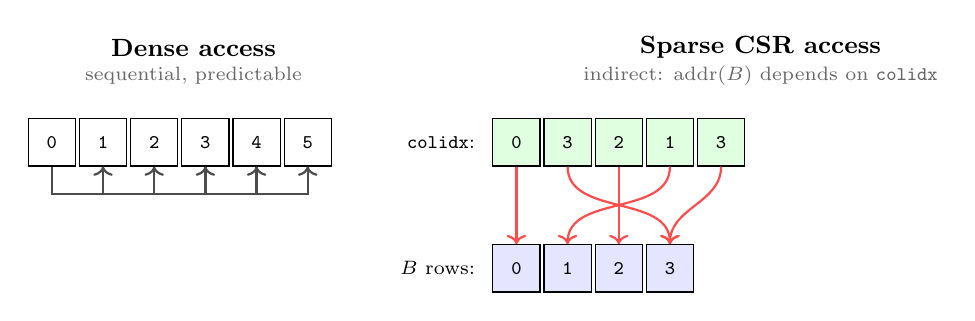
\begin{tikzpicture}[
      every node/.style={font=\small},
      cell/.style={draw, minimum width=6mm, minimum height=6mm, inner sep=0pt,
                   font=\scriptsize\ttfamily, anchor=center},
      acell/.style={draw, minimum width=6mm, minimum height=6mm, inner sep=0pt,
                    font=\scriptsize\ttfamily, fill=green!12},
      bcell/.style={draw, minimum width=6mm, minimum height=6mm, inner sep=0pt,
                    font=\scriptsize\ttfamily, fill=blue!10},
    ]
    % --- LEFT: dense access ---
    \node[font=\small\bfseries] at (1.8,2.6) {Dense access};
    \node[font=\scriptsize, text=black!60] at (1.8,2.25) {sequential, predictable};
    \foreach \i in {0,1,2,3,4,5} {
      \node[cell] (d\i) at (\i*0.65, 1.4) {\i};
    }
    \draw[->, thick, black!70] (d0.south) -- ++(0,-0.35) -| (d1.south);
    \draw[->, thick, black!70] (d1.south) -- ++(0,-0.35) -| (d2.south);
    \draw[->, thick, black!70] (d2.south) -- ++(0,-0.35) -| (d3.south);
    \draw[->, thick, black!70] (d3.south) -- ++(0,-0.35) -| (d4.south);
    \draw[->, thick, black!70] (d4.south) -- ++(0,-0.35) -| (d5.south);

    % --- RIGHT: sparse access ---
    \node[font=\small\bfseries] at (9.0,2.6) {Sparse CSR access};
    \node[font=\scriptsize, text=black!60] at (9.0,2.25)
      {indirect: addr$(B)$ depends on \texttt{colidx}};

    % colidx row
    \node[font=\scriptsize, anchor=east] at (5.5,1.4) {\texttt{colidx}:};
    \foreach \val [count=\i from 0] in {0,3,2,1,3} {
      \node[acell] (ci\i) at (5.9+\i*0.65, 1.4) {\val};
    }

    % B rows (destination) laid out as indexed rows
    \node[font=\scriptsize, anchor=east] at (5.5,-0.2) {$B$ rows:};
    \foreach \row in {0,1,2,3} {
      \node[bcell] (B\row) at (5.9+\row*0.65, -0.2) {\row};
    }

    % indirect pointer arrows: ci0 -> B0, ci1 -> B3, ci2 -> B2, ci3 -> B1, ci4 -> B3
    \draw[->, thick, red!70, out=-90, in=90] (ci0.south) to (B0.north);
    \draw[->, thick, red!70, out=-90, in=90] (ci1.south) to (B3.north);
    \draw[->, thick, red!70, out=-90, in=90] (ci2.south) to (B2.north);
    \draw[->, thick, red!70, out=-90, in=90] (ci3.south) to (B1.north);
    \draw[->, thick, red!70, out=-90, in=90] (ci4.south) to (B3.north);
  \end{tikzpicture}
  \caption{Memory access patterns in dense versus sparse CSR traversal. Dense
           access strides sequentially through contiguous addresses, so a
           prefetcher can fetch ahead. CSR access loads a column index from
           \texttt{colidx} first, then uses that value as an indirect pointer
           into $B$; the next address cannot be known until the previous load
           completes, which breaks prefetching and produces data-dependent
           cache misses.}
  \label{fig:access-pattern}
\end{figure}

\section{Sparse Matrix Storage Formats}

Several sparse matrix storage formats have been proposed; the choice of format
strongly affects the hardware control structure. Table~\ref{tab:sparse-formats}
summarises the most relevant formats and their suitability for hardware
acceleration.

\begin{table}[htbp]
  \centering
  \small
  \setlength{\tabcolsep}{2pt}
  \begin{tabular}{llp{4.0cm}p{3.5cm}}
  \toprule
  Format & Acronym & Description & Hardware suitability \\
  \midrule
  Coordinate list & COO &
    Stores (row, col, val) triplets unsorted or sorted by row.
    Simple to generate; requires sorting for efficient row-wise access. &
    High overhead per nonzero; poor for row-streaming hardware. \\[4pt]
  Compressed Sparse Row & CSR &
    Three arrays: \texttt{rowptr} ($M{+}1$ entries), \texttt{colidx} (NNZ),
    \texttt{values} (NNZ). Row bounds are contiguous. &
    Excellent for row-wise traversal; natural hardware FSM mapping. \\[4pt]
  ELLPACK & ELL &
    Pads each row to the maximum NNZ per row; stores in column-major order. &
    Good for regular sparsity; wastes storage and bandwidth when rows vary widely. \\[4pt]
  Block Compressed Sparse Row & BSR &
    Groups nonzeros into dense $r \times c$ blocks stored in CSR form. &
    High throughput on block-sparse matrices; unsuitable for unstructured sparsity. \\[4pt]
  Compressed Sparse Column & CSC &
    Transpose of CSR; columns are compressed. &
    Natural for column-wise access patterns; awkward for row-oriented output. \\
  \bottomrule
  \end{tabular}
  \caption{Comparison of common sparse matrix storage formats and their suitability
           for hardware acceleration.}
  \label{tab:sparse-formats}
\end{table}

\subsection{Why CSR Was Chosen}

Figure~\ref{fig:csr-layout} shows the CSR encoding of a small $4 \times 4$
sparse matrix. The three arrays \texttt{rowptr}, \texttt{colidx}, and
\texttt{values} together record exactly which nonzeros exist and where, with
no storage spent on the zero entries.

\begin{figure}[htbp]
  \centering
  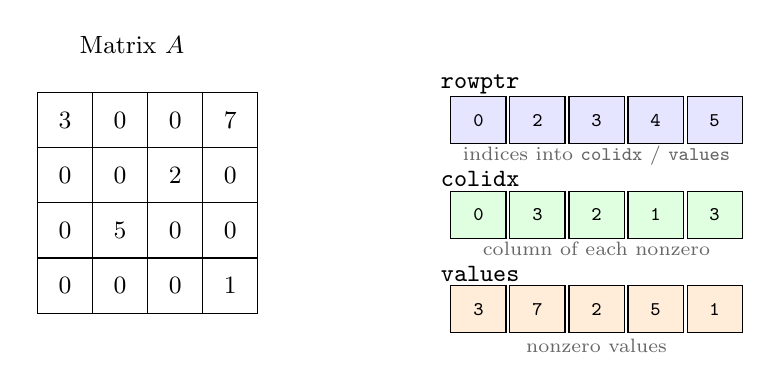
\begin{tikzpicture}[
      every node/.style={font=\small},
      mcell/.style={draw, minimum size=7mm, inner sep=0pt, anchor=center},
      acell/.style={draw, minimum width=7mm, minimum height=6mm, inner sep=0pt,
                    font=\scriptsize\ttfamily},
    ]
    % --- Matrix A ---
    \node[font=\small] at (-0.2,3) {Matrix $A$};
    \matrix (A) [matrix of nodes,
                 nodes={mcell},
                 column sep=-\pgflinewidth,
                 row sep=-\pgflinewidth,
                 nodes in empty cells] at (0,1) {
      3 & 0 & 0 & 7 \\
      0 & 0 & 2 & 0 \\
      0 & 5 & 0 & 0 \\
      0 & 0 & 0 & 1 \\
    };

    % --- rowptr ---
    \node[font=\small, anchor=west] at (3.6,2.5) {\texttt{rowptr}};
    \foreach \val [count=\i from 0] in {0,2,3,4,5} {
      \node[acell, fill=blue!10] (rp\i) at (4.2+\i*0.75, 2.05) {\val};
    }

    % --- colidx ---
    \node[font=\small, anchor=west] at (3.6,1.3) {\texttt{colidx}};
    \foreach \val [count=\i from 0] in {0,3,2,1,3} {
      \node[acell, fill=green!12] (ci\i) at (4.2+\i*0.75, 0.85) {\val};
    }

    % --- values ---
    \node[font=\small, anchor=west] at (3.6,0.1) {\texttt{values}};
    \foreach \val [count=\i from 0] in {3,7,2,5,1} {
      \node[acell, fill=orange!15] (vl\i) at (4.2+\i*0.75, -0.35) {\val};
    }

    % --- annotations ---
    \node[font=\scriptsize, anchor=north, text=black!60] at (5.7,1.85) {
      indices into \texttt{colidx} / \texttt{values}
    };

    \node[font=\scriptsize, anchor=north, text=black!60] at (5.7,0.63) {
      column of each nonzero
    };

    \node[font=\scriptsize, anchor=north, text=black!60] at (5.7,-0.6) {
      nonzero values
    };
  \end{tikzpicture}
  \caption{CSR encoding of a $4 \times 4$ sparse matrix with five nonzeros.
           \texttt{rowptr}[i] is the index of the first nonzero in row~$i$;
           row~$i$ owns entries \texttt{rowptr}[i] through
           \texttt{rowptr}[i{+}1]${-}1$ in both \texttt{colidx} and
           \texttt{values}. \texttt{rowptr}[M]${=}$NNZ by convention.}
  \label{fig:csr-layout}
\end{figure}

CSR was selected for this project because it maps directly onto the natural
execution order of row-wise SpMM. Gustavson's algorithm for sparse matrix
multiplication~\citep{gustavson1978} established that row-wise traversal of CSR
is asymptotically optimal for output-row-oriented computation, and that the row
pointer array provides $O(1)$ access to the start of each row's nonzero
sequence. Bell and Garland~\citep{bell_garland2009} demonstrated that CSR
remains the most widely supported format for both CPU and GPU SpMV/SpMM
implementations precisely because its memory layout matches the natural iteration
over output rows.

For a hardware FSM, the CSR structure offers a critical advantage: the bounds of
each row's nonzero segment are available with a single pointer read, and the
entire nonzero segment can be streamed sequentially from memory. There is no need
for global index sorting, block alignment padding, or two-dimensional address
translation. The firmware preparation cost is also low: generating CSR from a
list of nonzeros requires a single pass to count per-row nonzeros and a second
pass to write values and indices.

\section{Prior Work on SpMM Accelerators}

\subsection{OuterSPACE}

OuterSPACE~\citep{outerspace2018} targets the SpGEMM (sparse--sparse matrix
multiply) problem using an outer-product decomposition. Rather than traversing
CSR rows serially, it computes partial products for each nonzero column of $A$
and accumulates them into a merge tree. OuterSPACE achieves high throughput by
parallelising across columns of $A$ and using dedicated on-chip accumulators.
However, its design complexity (multiple merge stages, custom memory organisation,
and substantial on-chip storage for partial results) makes it unsuitable for
a constrained embedded SoC design such as the present work.

\subsection{SpArch}

SpArch~\citep{sparch2020} also targets sparse--sparse computation, focusing on
the merger phase that reduces partial products to a final output. It introduces
a condenser that reorganises partial products to maximise row-merger bandwidth.
SpArch demonstrates that the merger step, not the multiplication step, typically
dominates sparse--sparse computation time. While SpArch's insights are instructive,
its target workload (sparse--sparse) is more general than SpMM (sparse--dense),
and the design's reliance on complex inter-row scheduling is not well matched
to the CSR traversal structure exploited in this project.

\subsection{ExTensor}

ExTensor~\citep{extensor2019} generalises sparse computation to higher-order
tensors and introduces the concept of intersection hardware to skip pairs of
zero operands before they reach the multiplier array. It demonstrates that
intersection-based skipping can significantly improve efficiency over na\"ive
zero-skipping by avoiding the memory read entirely when a nonzero pair is absent.
The present design achieves a weaker form of zero-skipping through CSR itself:
zero rows of $A$ produce no nonzero traversal steps, and the CSR column index
array only points to nonzero entries. Full intersection logic would require more
complex comparison hardware across both $A$ and $B$.

\subsection{SIGMA}

SIGMA~\citep{sigma2020} targets the sparse-weight GEMM that arises during
DNN training after unstructured pruning. It uses a flexible
\textit{Forwarding Adder Network} (FAN) as a reduction tree whose connectivity
is reconfigured at runtime to match the nonzero pattern of the weight matrix.
SIGMA demonstrates that hardware-reconfigurable reduction topologies can match
the irregular sparsity structure of training-time gradients, but the resource
overhead of a general FAN is substantial and is not appropriate for a
small-scale FPGA SoC.

\subsection{Positioning This Work}

All of the accelerators reviewed above target substantially larger throughput
regimes, more aggressive scheduling mechanisms, and dedicated memory hierarchies
that are not available on a Cyclone V FPGA. The present project is intentionally
different in scope: it is a tightly integrated, reproducible, RTL-level
PicoRV32-attached accelerator with shared on-chip memory, explicit MMIO control,
and a staged optimisation narrative. The contribution is therefore not a new
scheduling algorithm or interconnect topology, but rather a complete and clearly
characterised implementation that demonstrates how far CSR SpMM can be pushed on
a constrained RISC-V FPGA platform by aligning the memory format, datapath, and
quantisation strategy with the dominant cost of the workload.

\section{Hardware Platform Alternatives}

\subsection{CPU}

General-purpose CPUs offer the highest programmability but handle SpMM
inefficiently. The irregular access pattern defeats prefetching and out-of-order
speculation. Cache misses to scattered rows of $B$ dominate execution time at
large problem sizes. On a small in-order soft-core such as PicoRV32, there is
no out-of-order machinery or data cache at all, so every operand fetch to BRAM
incurs the full BRAM latency.

\subsection{GPU}

GPUs achieve high SpMM throughput by exploiting massive parallelism and high
memory bandwidth. Libraries such as cuSPARSE implement carefully tuned kernels
for CSR SpMM on modern GPUs~\citep{bell_garland2009}. However, GPUs require
substantial power (100--400\,W for a discrete card), DRAM for large batch sizes,
and complex runtime support stacks. They are not viable for an embedded SoC
implementation.

\subsection{FPGA}

FPGAs offer a middle ground: custom datapath parallelism, flexible on-chip
memory organisation, and far lower power than a GPU~\citep{nurvitadhi2017}.
The Cyclone V FPGA on the DE1-SoC provides on-chip M10K BRAM blocks, DSP
multiplier-accumulator blocks, and configurable logic elements that can be
combined into a bespoke SpMM datapath without the overhead of a general-purpose
instruction set. FPGA fabric also allows the memory interface to be tailored
exactly to the access pattern of CSR traversal, eliminating unnecessary
transactions.

\subsection{ASIC}

A custom ASIC would deliver the highest throughput and lowest power for SpMM,
but development cost, fabrication lead time, and inflexibility make ASICs
impractical for a final-year design project. The FPGA is the natural choice
for prototyping and validating a custom accelerator architecture before any
ASIC commitment~\citep{nurvitadhi2017}.

\section{INT8 Quantisation}

\subsection{Motivation}

Quantisation reduces the numerical precision of stored values, decreasing memory
footprint and potentially increasing arithmetic throughput~\citep{jacob2018,
nagel2021}. For SpMM specifically, quantisation affects the bottleneck directly:
if operands are stored as 8-bit integers rather than 32-bit floats, four times as
many values can be fetched per memory transaction. Given that SpMM is
memory-bandwidth-limited (Section~2.2), this is a particularly powerful
optimisation.

\subsection{Symmetric Linear Quantisation}

The project adopts runtime symmetric linear quantisation. Given a vector $\mathbf{v}$
of full-precision values, the maximum absolute value $v_{\max} = \max_i |v_i|$
is computed, and each value is mapped to a signed 8-bit integer by
\begin{equation}
  q_i = \mathrm{clip}\!\left(\operatorname{round}\!\left(
          \frac{v_i}{v_{\max}} \cdot 127 \right),\,-127,\,127\right),
  \label{eq:quant}
\end{equation}
where the scale factor is $s = v_{\max} / 127$. Reconstruction uses
$\hat{v}_i = q_i \cdot s$, so the quantisation error is bounded by
$|e_i| \leq s/2$. Symmetric quantisation was preferred over asymmetric because
it eliminates the need for a zero-point offset in the inner MAC loop, simplifying
the hardware accumulation logic.

\subsection{Effect on Memory Traffic}

In the un-packed baseline, one 32-bit memory word carries one operand. With INT8
packing, one 32-bit word carries four operands. For a $TN = 8$ tile, filling the
local $B$ segment buffer therefore falls from eight RAM reads to two RAM reads in
the common case. Since RAM read latency is the dominant term in the accelerator's
cycle budget (Section~\ref{ch:design}), this 4$\times$ reduction in operand fetch
count translates directly into a large cycle reduction.

\subsection{Accumulation Precision}

INT8 accumulation into INT8 is insufficient for most practical workloads:
a sum of $K$ products of INT8 values each up to $\pm 127$ can reach
$\pm 127^2 \cdot K = \pm 16{,}129 K$, which overflows INT8 and INT16 even for
moderate $K$. The present design therefore accumulates into INT32, which
can represent sums of up to $2^{31}/16{,}129 \approx 133{,}000$ elements before
overflow. This matches the widely adopted practice of INT8$\times$INT8 with INT32
accumulation as described by Jacob et al.~\citep{jacob2018}.

\section{Roofline Analysis and Design Implications}

The roofline model~\citep{williams2009roofline} characterises whether a kernel
is compute-bound (throughput limited by the peak FLOP rate) or
memory-bound (throughput limited by available bandwidth). The position of a
kernel on the roofline is determined by its \emph{arithmetic intensity}: the
ratio of floating-point operations to bytes of off-chip data movement.

For the baseline accelerator on a Cyclone~V device operating at 50\,MHz with a
$TN = 8$ parallel MAC array, the peak throughput is
\[
  T_{\mathrm{peak}} = 8 \;\text{MACs/cycle} \;\times\; 50 \;\text{MHz}
                    = 400 \;\text{MMACs/s}.
\]
With 32-bit operands, the on-chip BRAM bandwidth for a single dual-port block is
two 32-bit reads per cycle, giving 400\,MB/s. For $TN = 8$ fully utilised,
eight reads per cycle are needed to fill the $B$ segment, but the accelerator
shares a single port with the CPU and issues reads sequentially. Thus, even at
$TN = 8$, the MAC units are stalled waiting for RAM reads approximately
$\frac{8}{1} = 8\times$ more than they are computing. This analysis confirms that
the accelerator is memory-bandwidth-limited in the baseline configuration.

INT8 packing reduces the number of required reads from eight to two, moving the
design's operating point along the roofline x-axis towards the compute-bound
region. This is the theoretical basis for the large speedup gain observed in the
INT8 stage, and is consistent with the $2.18\times$ cycle reduction observed
across the 12-case sweep. Figure~\ref{fig:roofline} illustrates the shift:
the baseline design sits well to the left of the roofline knee, where
throughput is bounded by memory bandwidth, and INT8 packing moves it towards
the compute-bound plateau.

\begin{figure}[htbp]
  \centering
  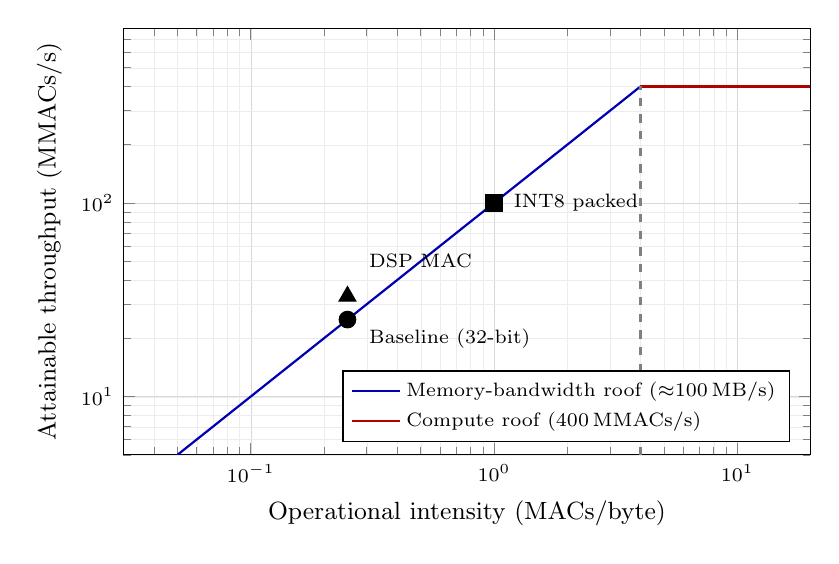
\begin{tikzpicture}
    \begin{axis}[
      width=0.85\linewidth, height=7cm,
      xmode=log, ymode=log,
      xlabel={Operational intensity (MACs/byte)},
      ylabel={Attainable throughput (MMACs/s)},
      xmin=0.03, xmax=20,
      ymin=5, ymax=800,
      grid=both,
      major grid style={line width=.1pt,draw=gray!30},
      minor grid style={line width=.05pt,draw=gray!15},
      legend pos=south east,
      legend cell align={left},
      legend style={font=\scriptsize},
      tick label style={font=\scriptsize},
      label style={font=\small},
    ]
      % Memory roof: throughput = BW * OI; BW = 100 MB/s (one 32-bit read per cycle @ 50 MHz = 200 MB/s; but shared => 100)
      % So throughput (MMACs/s) = 100 * OI (if OI in MACs/byte)
      \addplot[domain=0.03:4, samples=2, thick, blue!70!black] {100*x};
      \addlegendentry{Memory-bandwidth roof ($\approx$100\,MB/s)};

      % Compute roof: 400 MMACs/s peak
      \addplot[domain=4:20, samples=2, thick, red!70!black] {400};
      \addlegendentry{Compute roof (400\,MMACs/s)};

      % Connector at the knee (x=4)
      \addplot[domain=4:4, samples=2, thick, dashed, gray] coordinates {(4,5)(4,400)};

      % Baseline point: OI ~ 0.25, throughput limited to 25 MMACs/s
      \addplot[only marks, mark=*, mark size=3pt, black] coordinates {(0.25,25)};
      \node[anchor=west, font=\scriptsize] at (axis cs:0.28,20) {Baseline (32-bit)};

      % DSP MAC point: same OI (memory unchanged), slightly better arithmetic
      \addplot[only marks, mark=triangle*, mark size=3.5pt, black] coordinates {(0.25,33)};
      \node[anchor=west, font=\scriptsize] at (axis cs:0.28,50) {DSP MAC};

      % INT8 point: OI ~ 1.0 (4x more operands per byte), throughput ~100 MMACs/s
      \addplot[only marks, mark=square*, mark size=3pt, black] coordinates {(1.0,100)};
      \node[anchor=west, font=\scriptsize] at (axis cs:1.1,100) {INT8 packed};
    \end{axis}
  \end{tikzpicture}
  \caption{Roofline interpretation of the three accelerator stages on the
           Cyclone~V platform. The baseline and DSP-enhanced designs sit on
           the memory-bandwidth roof: arithmetic throughput is capped by
           operand fetch, so widening the MAC array yields only a small gain.
           INT8 packing raises the operational intensity by a factor of four
           (four operands per 32-bit word), shifting the design rightward and
           upward along the bandwidth roof towards the compute-bound region.}
  \label{fig:roofline}
\end{figure}

\chapter{System Design and RISC-V Platform}
\label{ch:platform}

\section{Deployment Context and Platform Overview}

The implemented design targets the Terasic DE1-SoC development board, which
carries a Cyclone~V 5CSEMA5F31C6 FPGA device~\citep{de1soc_manual}. The SoC
is synthesised entirely into the FPGA fabric; it does not use the hard ARM
Cortex-A9 processor on the DE1-SoC's HPS. This choice keeps the design
self-contained in the FPGA, makes cycle-level timing directly controllable
through HDL, and avoids the complexity of AXI bridges, Linux boot, and HPS
memory management.

The entire benchmark path executes on-chip: firmware, CSR arrays, dense matrix
$B$, and output matrix $C$ all reside in the shared 64\,KB dual-port block RAM.
This simplifies the memory system and makes cycle comparisons easier to interpret
at the cost of limiting the benchmark problem sizes to those that fit comfortably
in on-chip memory. The design runs from the 50\,MHz on-board oscillator.

Figure~\ref{fig:soc-block} shows the top-level block diagram of the implemented
SoC.

\begin{figure}[htbp]
    \centering
    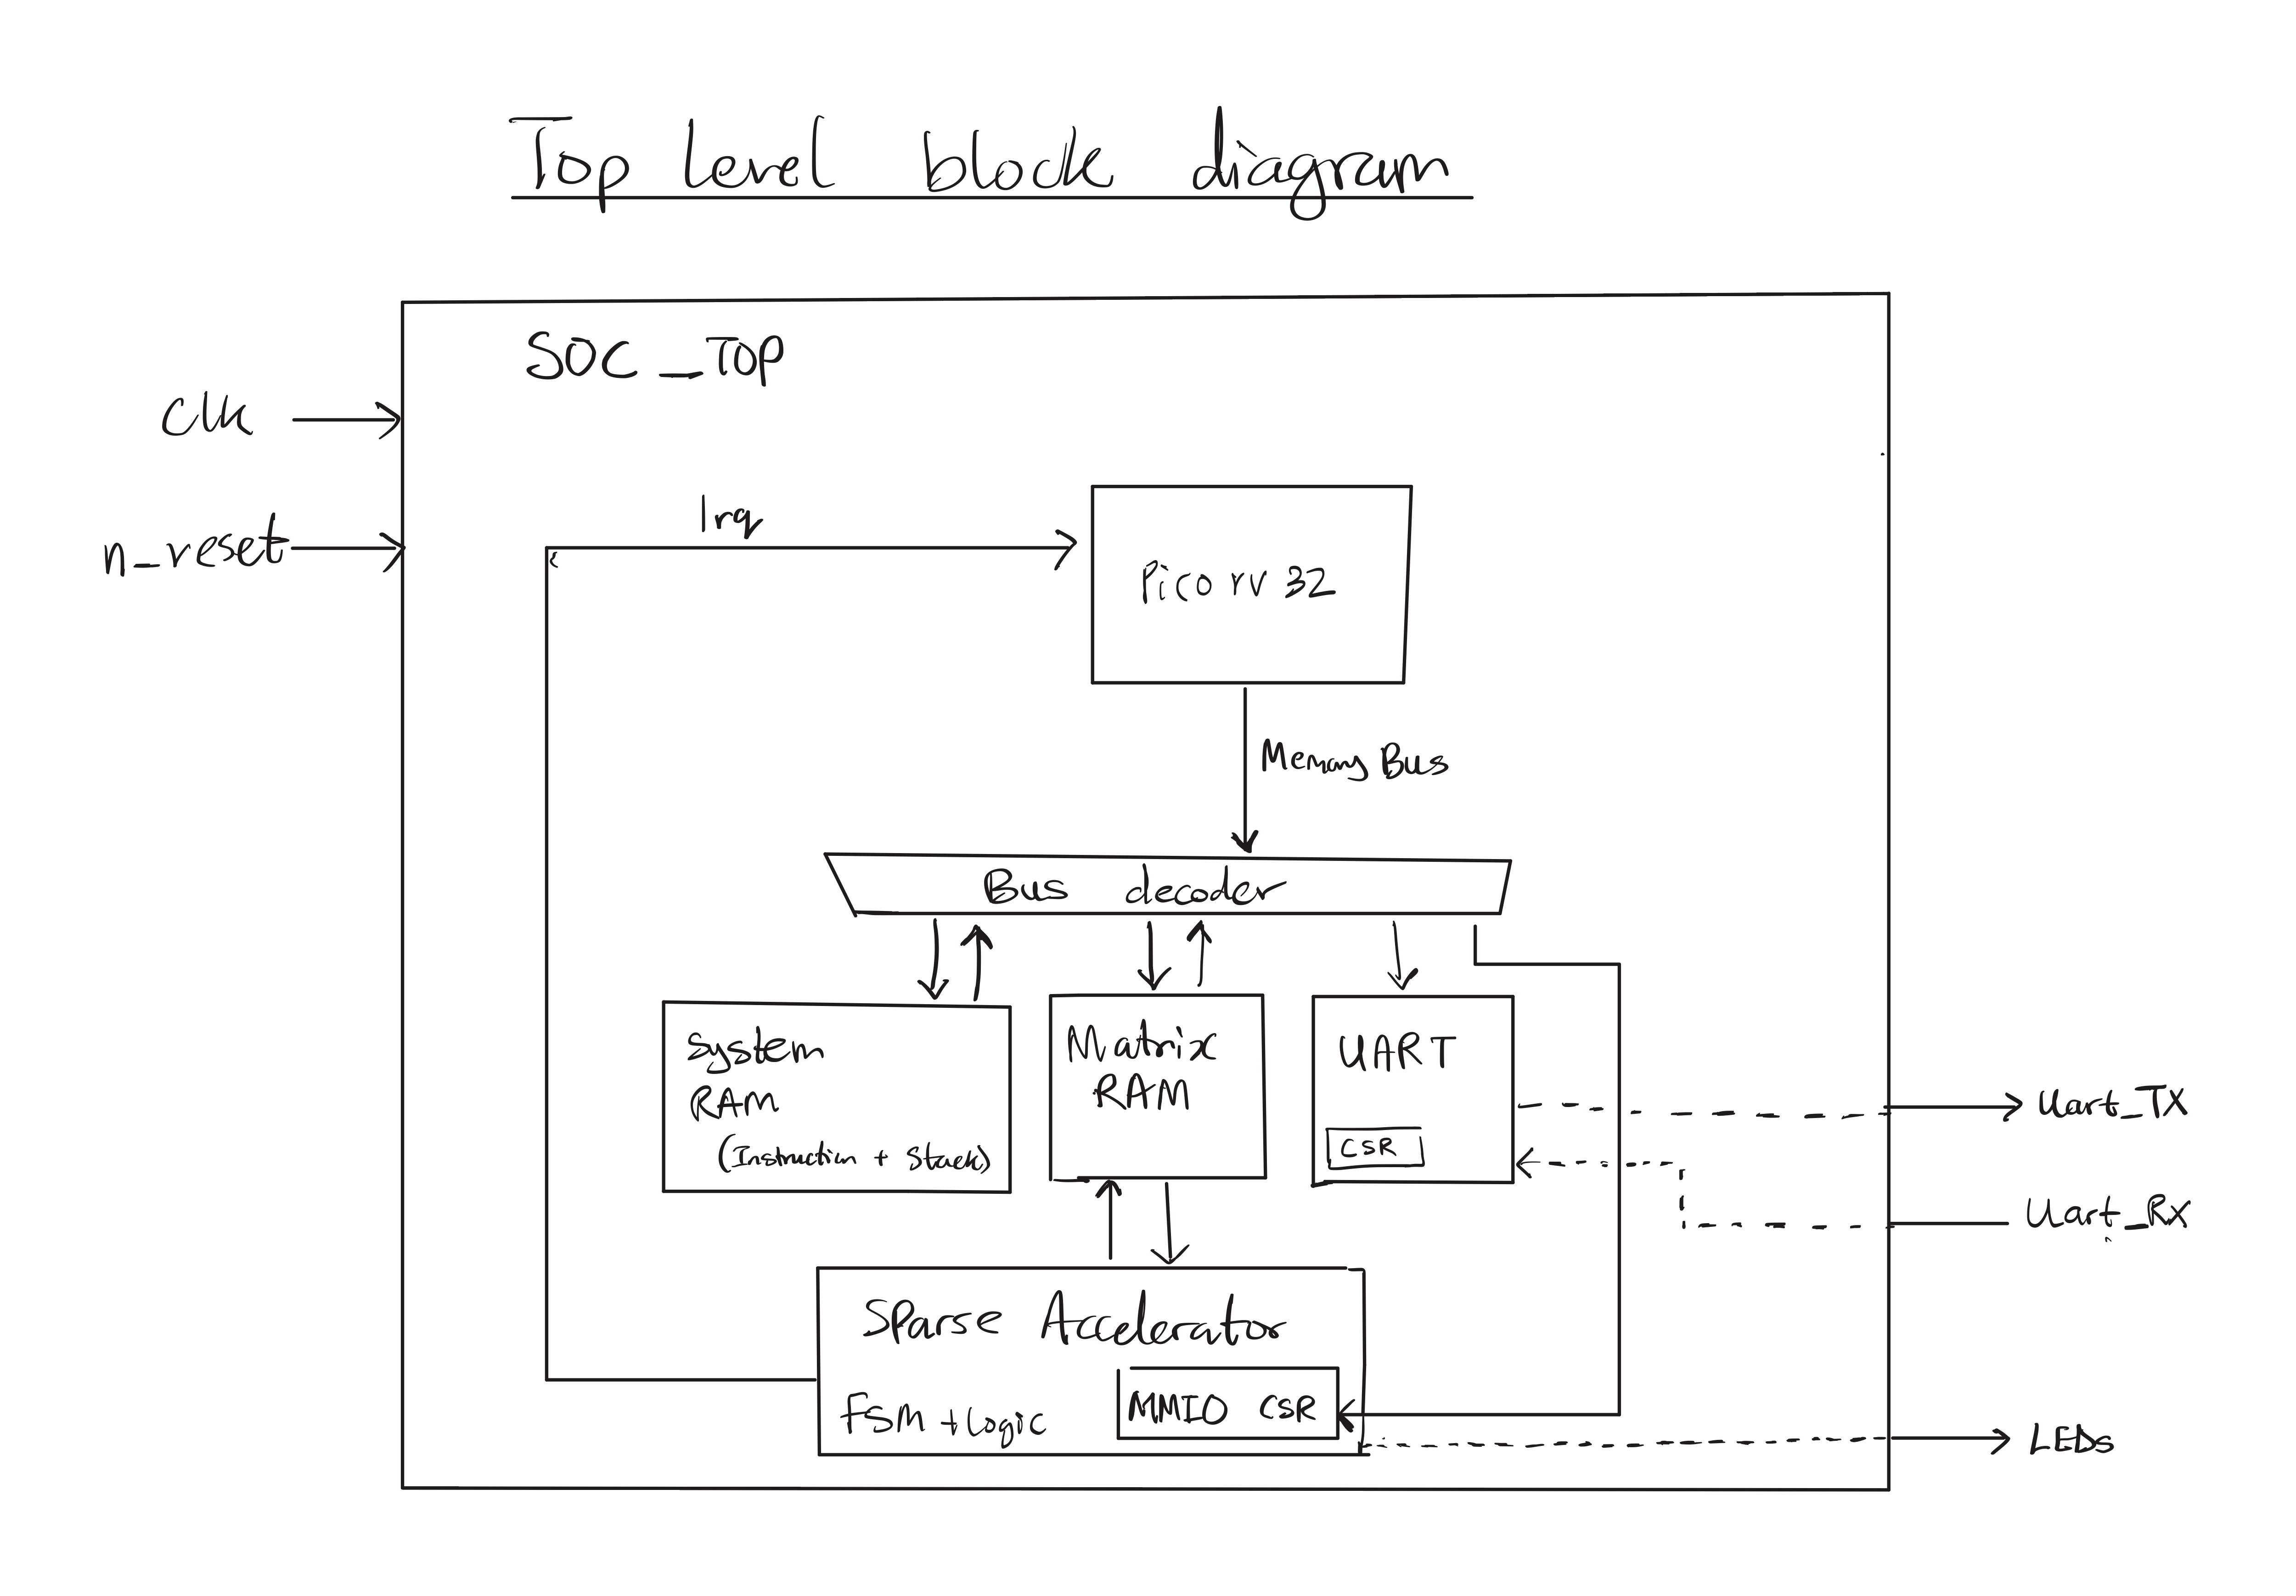
\includegraphics[width=1\textwidth]{top_block_dia.jpg}
    \caption{Top-level RISC-V SoC block diagram showing PicoRV32 CPU, shared
             dual-port RAM, SpMM accelerator, UART peripheral, and GPIO
             interface, all connected via memory-mapped I/O.}
    \label{fig:soc-block}
\end{figure}

\section{Target FPGA: Cyclone V Resources}

The Cyclone~V 5CSEMA5F31C6 device provides the following key resources
\citep{cyclonev_handbook}:

\begin{table}[htbp]
  \centering
  \small
  \begin{tabular}{lrr}
  \toprule
  Resource & Total available & Used (estimated) \\
  \midrule
  Adaptive Logic Modules (ALMs) & 32,070 & $\approx$5,000 (16\%) \\
  Logic registers & 128,280 & $\approx$8,000 (6\%) \\
  M10K memory blocks (10\,Kbit each) & 397 & $\approx$20 (5\%) \\
  DSP 18$\times$18 multiplier blocks & 87 & $\approx$8 (9\%) \\
  I/O pins & 457 & --- \\
  \bottomrule
  \end{tabular}
  \caption{Cyclone~V 5CSEMA5F31C6 resource availability and estimated
           design utilisation. Final synthesis numbers are pending completion
           of the Quartus timing closure study.}
  \label{tab:fpga-resources}
\end{table}

The M10K blocks each provide 10\,Kbits (approximately 1.25\,KB) of configurable
on-chip memory~\citep{intel_m10k}. At true-dual-port configuration with
32-bit-wide ports, each M10K can hold 256 words. The 64\,KB BRAM used in this
design requires approximately 16 M10K blocks in a cascaded configuration, leaving
substantial BRAM capacity for other purposes. The DSP blocks implement
18$\times$18-bit two's-complement signed multipliers followed by a dedicated
accumulator register, making them well-suited to INT32 MAC operations when
configured appropriately~\citep{intel_dsp_blocks}.

\section{PicoRV32 Host Processor}

The host processor is PicoRV32~\citep{picorv32}, a compact RV32IM soft-core
implementing the RISC-V base integer instruction set with the hardware integer
multiply extension (M)~\citep{riscv_isa}. PicoRV32 was chosen because:
\begin{itemize}
  \item it is small (approximately 700--1000 ALMs), leaving adequate FPGA fabric
        for the accelerator and memory;
  \item it supports the \texttt{rdcycle} performance counter CSR natively, which
        is used for all cycle-accurate timing measurements; and
  \item it exposes a simple memory bus (valid/ready handshake with address, data,
        and write-enable signals) that maps directly onto the SoC interconnect.
\end{itemize}

PicoRV32 is an in-order, non-pipelined core. It issues one instruction at a time,
incurring full stall cycles on every load instruction. For instructions that access
the synchronous dual-port BRAM, the latency is one clock cycle after the address
is presented. This is important for interpreting accelerator speedups: the CPU
software baseline is a simple in-order core with no caching and no out-of-order
execution, making the accelerator's advantage larger than it would be against a
modern superscalar CPU.

The M extension provides hardware 32$\times$32 integer multiply and divide. The
software SpMM reference uses \texttt{MUL} instructions for the inner-loop
multiply--accumulate. Without the M extension, PicoRV32 would fall back to a
software multiply routine that is typically 10--30$\times$ slower, which would
artificially inflate speedup numbers. The M extension is therefore required for
a credible software baseline.

\section{System Memory Map and Bus Architecture}

\subsection{Bus Protocol}

The SoC interconnect uses the native PicoRV32 memory bus: a
valid/ready handshake with a 32-bit address bus, a 32-bit bidirectional data
bus, a 4-bit byte-enable signal, and a read/write indicator. The bus is
synchronous to the 50\,MHz system clock. Access latency is a single cycle for
BRAM (using the BRAM's registered output) and combinatorial for MMIO registers.

\subsection{Address Space}

Table~\ref{tab:system-memory-map} summarises the complete system memory map.

\begin{table}[htbp]
  \centering
  \small
  \begin{tabular}{lp{3.0cm}p{5.5cm}}
  \toprule
  Address range & Peripheral & Purpose \\
  \midrule
  \texttt{0x0000\_0000--0x0000\_FFFF} & On-chip RAM (64\,KB) &
    Firmware code, stack, CSR arrays (\texttt{rowptr}, \texttt{colidx},
    \texttt{values}), dense matrix $B$, output matrix $C$ \\[4pt]
  \texttt{0x1000\_0000--0x1000\_00FF} & SpMM accelerator MMIO &
    Configuration registers, control, and status \\[4pt]
  \texttt{0x2000\_0000--0x2000\_000F} & GPIO &
    LED output, switch and button input, seven-segment display \\[4pt]
  \texttt{0x2000\_0100--0x2000\_01FF} & UART (\texttt{simpleuart}) &
    Serial output for UART benchmark reporting at 115200\,baud \\
  \bottomrule
  \end{tabular}
  \caption{System memory map of the implemented RISC-V SoC.}
  \label{tab:system-memory-map}
\end{table}

\subsection{Dual-Port BRAM Organisation}

The 64\,KB on-chip RAM is implemented as an Altera \texttt{altsyncram}
true-dual-port memory with 32-bit-wide ports. Port~A is connected exclusively
to the PicoRV32 CPU and supports byte-granular write-enable (4-bit byte
mask). Port~B is connected exclusively to the SpMM accelerator and uses
32-bit word-granular access. This organisation allows the CPU and accelerator
to access different addresses simultaneously without arbitration, which is
important during data preparation phases where the CPU writes CSR arrays
while the previous accelerator output is being read out over UART.

Both ports share the same underlying memory array, so concurrent accesses to the
same address produce undefined results. The firmware scheduling ensures that the
CPU does not write to active accelerator buffers during an accelerator run.

\section{Accelerator MMIO Register Interface}

The accelerator exposes its control and configuration through a bank of
memory-mapped registers accessible from the CPU at addresses
\texttt{0x1000\_0000}--\texttt{0x1000\_002C}. Table~\ref{tab:mmio-regs} lists
the complete register set.

\begin{table}[htbp]
  \centering
  \small
  \begin{tabular}{llp{6.2cm}}
  \toprule
  Offset & Name & Description \\
  \midrule
  \texttt{0x00} & \texttt{CTRL} &
    Control register: bit 0 = \texttt{start} (self-clearing pulse),
    bit 1 = \texttt{clear\_done}, bit 2 = \texttt{irq\_en}
    (reserved; polling used), bit 3 = \texttt{relu\_en},
    bit 4 = \texttt{int8\_mode} \\[4pt]
  \texttt{0x04} & \texttt{STATUS} &
    Status register: bit 0 = \texttt{busy}, bit 1 = \texttt{done} \\[4pt]
  \texttt{0x08} & \texttt{M} & Number of rows in $A$ and $C$ \\
  \texttt{0x0C} & \texttt{N} & Number of columns in $B$ and $C$ (dense width) \\
  \texttt{0x10} & \texttt{K} & Number of columns in $A$ / rows in $B$ \\
  \texttt{0x14} & \texttt{A\_VAL\_BASE} & Base address of CSR \texttt{values} array \\
  \texttt{0x18} & \texttt{A\_ROW\_BASE} & Base address of CSR \texttt{rowptr} array \\
  \texttt{0x1C} & \texttt{A\_COL\_BASE} & Base address of CSR \texttt{colidx} array \\
  \texttt{0x20} & \texttt{B\_BASE} & Base address of dense matrix $B$ (row-major) \\
  \texttt{0x24} & \texttt{C\_BASE} & Base address of output matrix $C$ (row-major) \\
  \texttt{0x28} & \texttt{NNZ} & Total number of nonzeros in $A$ \\
  \bottomrule
  \end{tabular}
  \caption{SpMM accelerator MMIO register map. All registers are 32-bit
           word-aligned. Base addresses are byte addresses into the shared
           64\,KB RAM.}
  \label{tab:mmio-regs}
\end{table}

The \texttt{start} bit is asserted as a single-cycle pulse from the CPU; the
accelerator captures it and immediately transitions from \texttt{IDLE} to its
computation sequence. The \texttt{done} flag is asserted by the accelerator when
all output rows have been written to RAM and remains asserted until the CPU
writes the \texttt{clear\_done} bit. The interrupt-enable bit exists in the
hardware but the firmware uses polling; the interrupt is reserved for future use.

\section{Expected Accelerator Function}

At system level, the accelerator is specified to:
\begin{enumerate}
  \item read matrix dimensions $M$, $N$, $K$, and NNZ from MMIO registers;
  \item interpret matrix $A$ in CSR form using the three base-address registers;
  \item read dense matrix $B$ from shared RAM in row-major layout;
  \item compute $C = A \times B$ using tiled parallel MAC operations;
  \item optionally apply element-wise ReLU on each output element before writeback
        when \texttt{relu\_en} is asserted; and
  \item signal completion by asserting \texttt{STATUS.done} and releasing
        \texttt{STATUS.busy}.
\end{enumerate}

The optional INT8 mode (\texttt{CTRL.int8\_mode}) instructs the accelerator to
interpret the \texttt{values} array and matrix $B$ as packed INT8 rather than
INT32, sign-extending each byte to 32 bits before multiplication.

\section{System-Level Requirements and Constraints}

The main requirements and constraints that shaped the design are:

\begin{itemize}
  \item \textbf{No external memory interface.} The design must operate
        entirely from on-chip BRAM, avoiding the complexity and latency of an
        SDRAM or DDR controller. This bounds the benchmark problem sizes but
        keeps the system self-contained and the cycle counts interpretable.

  \item \textbf{Simple MMIO control.} The accelerator must be usable from
        bare-metal firmware without an operating system or DMA engine. Register
        writes and a polling loop are sufficient.

  \item \textbf{Dense-dimension tiling with $TN = 8$.} The design exploits
        parallelism across output columns in fixed-width tiles. A tile width of
        eight was chosen to provide meaningful parallelism (8 simultaneous MACs)
        without exceeding Cyclone V DSP and BRAM routing limits.

  \item \textbf{Reproducible cycle-accurate benchmarking.} The firmware
        benchmark suite must be deterministic (fixed seeds), self-verifying
        (element-by-element comparison), and cycle-accurate (using
        \texttt{rdcycle}).

  \item \textbf{Practical memory layout.} CSR arrays, matrix $B$, and output
        matrix $C$ must all fit in the 64\,KB shared RAM alongside the firmware
        stack and code. This constrains the maximum problem size to approximately
        $M = K = 64$, $N = 32$, with the exact bound depending on NNZ.
\end{itemize}

These constraints explain the deliberate simplicity of the polling completion
model, the choice of $TN = 8$ rather than a wider datapath, and the decision to
generate benchmark data at runtime rather than loading it from external storage.

\chapter{Accelerator Design and Optimisation Methods}
\label{ch:design}

\section{Design Philosophy and Architecture}

The accelerator was shaped by the execution structure of CSR SpMM rather
than adapted from a generic dense-matrix template. CSR SpMM has three
distinct computational phases (row-bound loading, nonzero streaming, and
dense tile accumulation), and each phase has a different memory and
control-flow character. Any hardware design that treats them as a single
monolithic pipeline inevitably over-engineers one phase and underserves
another, so the architecture instead separates concerns explicitly: a
control finite state machine (\texttt{accel\_ctrl}) walks the CSR structure
and sequences RAM accesses, while a datapath (\texttt{accel\_datapath})
performs the parallel multiply--accumulate and manages the local tile
buffers. This split follows standard digital design
practice~\citep{sze2017} and, more importantly, allows each half of the
accelerator to be verified independently in simulation before integration.

The top-level module (\texttt{accel\_top}) wraps these two blocks together
with an MMIO front-end that decodes the PicoRV32 memory bus and exposes the
configuration interface of Table~\ref{tab:mmio-regs}. The accelerator
reaches shared memory through Port~B of the dual-port BRAM, a 32-bit
word-granular port with one cycle of registered read latency. All RAM
accesses are therefore scheduled as paired issue/consume phases separated
by exactly one clock cycle, which gives the controller a deterministic
latency model and removes the need for a stall/ready handshake.

\section{Baseline Datapath}

The datapath is parameterised by a tile width $TN = 8$ (the number of
output columns processed in parallel), a maximum row count
$M_{\mathrm{max}} = 64$, and a 32-bit signed operand width. Its behaviour
depends on two local buffers whose sizing is critical to performance. The
first, \texttt{B\_Seg}, is an eight-element array of signed 32-bit values
that holds the current row segment of dense matrix $B$: for every nonzero
$a_{ij}$ the controller fills \texttt{B\_Seg} with
$B[j,\,c_0:c_0{+}TN]$ before enabling the MAC array. The second,
\texttt{C\_Tile}, is an $M_{\mathrm{max}} \times TN$ array of signed 32-bit
partial sums that accumulates the output tile for all rows of $C$
simultaneously within the current tile column $[c_0, c_0{+}TN)$. Using a
flat two-dimensional accumulator rather than per-row registers avoids
writeback/restore cycles when nonzeros from different rows touch the same
tile column, which is the common case in realistically distributed sparse
matrices. The C-tile is implemented as a 512-register fabric array rather
than BRAM; on the Cyclone~V each ALM carries two registers, so the tile
consumes roughly 256 ALMs, well within the budget of the target device.

For each nonzero $a = A[i,k]$ the controller asserts \texttt{mac\_en},
\texttt{mac\_row} $= i$, and \texttt{mac\_a} $= a$, and the datapath issues
eight simultaneous signed multiply--accumulate operations:
\[
  \texttt{C\_Tile}[i][c] \;\mathrel{+}=\; \texttt{mac\_a} \,\times\,
  \texttt{B\_Seg}[c] \qquad c = 0, 1, \ldots, TN{-}1.
\]
This is the key mapping that gives the accelerator its parallelism: a
single nonzero in $A$ interacts with an entire row segment of $B$, so one
issue cycle produces $TN$ output updates. The parallelism is across the
dense output dimension, where the workload is regular, rather than along
the sparse dimension, where it is not. When all rows have been processed
in the current tile column, the C-tile is streamed back to shared RAM row
by row; if \texttt{CTRL.relu\_en} is asserted, an element-wise
$\max(0, \cdot)$ is applied to each value on writeback, making the
accelerator directly usable as the fully-connected layer of a neural
network inference pipeline.

\section{Control FSM}
\label{sec:fsm}

The control FSM is the most intricate component of the design. It drives
all address generation, RAM sequencing, nonzero traversal, and tile
management, and cycles through the phases listed in
Table~\ref{tab:fsm-states}; the sub-phase indices within
\texttt{ROW\_LOAD} and \texttt{NZ\_FETCH} exist specifically to cover the
one-cycle registered RAM latency. The simplified state-level view is
shown in Figure~\ref{fig:accel-fsm}.

\begin{table}[htbp]
  \centering
  \small
  \begin{tabular}{p{3.8cm}p{8.6cm}}
  \toprule
  State & Action \\
  \midrule
  \texttt{IDLE} &
    Wait for \texttt{start} pulse. Load $M$, $N$, $K$, NNZ, and base
    addresses from the MMIO register snapshot. \\[4pt]
  \texttt{INIT\_TILE\_CLEAR} &
    Clear all entries of \texttt{C\_Tile} to zero in preparation for the
    first tile column (one row per cycle, $M_{\mathrm{max}}$ cycles). \\[4pt]
  \texttt{ROW\_LOAD} &
    Load the CSR row bounds for the current row $i$: issue reads for
    \texttt{rowptr[i]} and \texttt{rowptr[i+1]}; handle the registered RAM
    output latency using sub-phases \texttt{ROW\_PHASE\_0/1/2}. \\[4pt]
  \texttt{NZ\_FETCH} &
    For each nonzero in \texttt{[rowptr[i], rowptr[i+1])}: read
    \texttt{values[p]} and \texttt{colidx[p]} and compute the starting
    address of $B[\texttt{col},:]$ for the current tile. Sub-phases
    \texttt{NZ\_PHASE\_0}--\texttt{NZ\_PHASE\_4} handle RAM latency and
    address arithmetic. \\[4pt]
  \texttt{MAC} &
    Fill \texttt{B\_Seg} with $TN$ consecutive values from $B$ (one per
    clock in INT32 mode, two reads total in INT8 mode), then assert
    \texttt{mac\_en} for one cycle to update \texttt{C\_Tile}. \\[4pt]
  \texttt{NEXT\_ROW} &
    Increment the row index. If more rows remain in this tile column, loop
    to \texttt{ROW\_LOAD}; otherwise proceed to \texttt{WRITE\_TILE}. \\[4pt]
  \texttt{WRITE\_TILE} &
    Write all $M \times TN$ entries of \texttt{C\_Tile} back to shared RAM
    (with optional ReLU). Advance the tile column offset by $TN$; if more
    tile columns remain, clear \texttt{C\_Tile} and loop to
    \texttt{ROW\_LOAD}, otherwise proceed to \texttt{DONE}. \\[4pt]
  \texttt{DONE} &
    Assert \texttt{STATUS.done} and release \texttt{STATUS.busy}; return
    to \texttt{IDLE} when \texttt{clear\_done} is asserted by the CPU. \\
  \bottomrule
  \end{tabular}
  \caption{Accelerator FSM states and their actions.}
  \label{tab:fsm-states}
\end{table}

\begin{figure}[htbp]
  \centering
  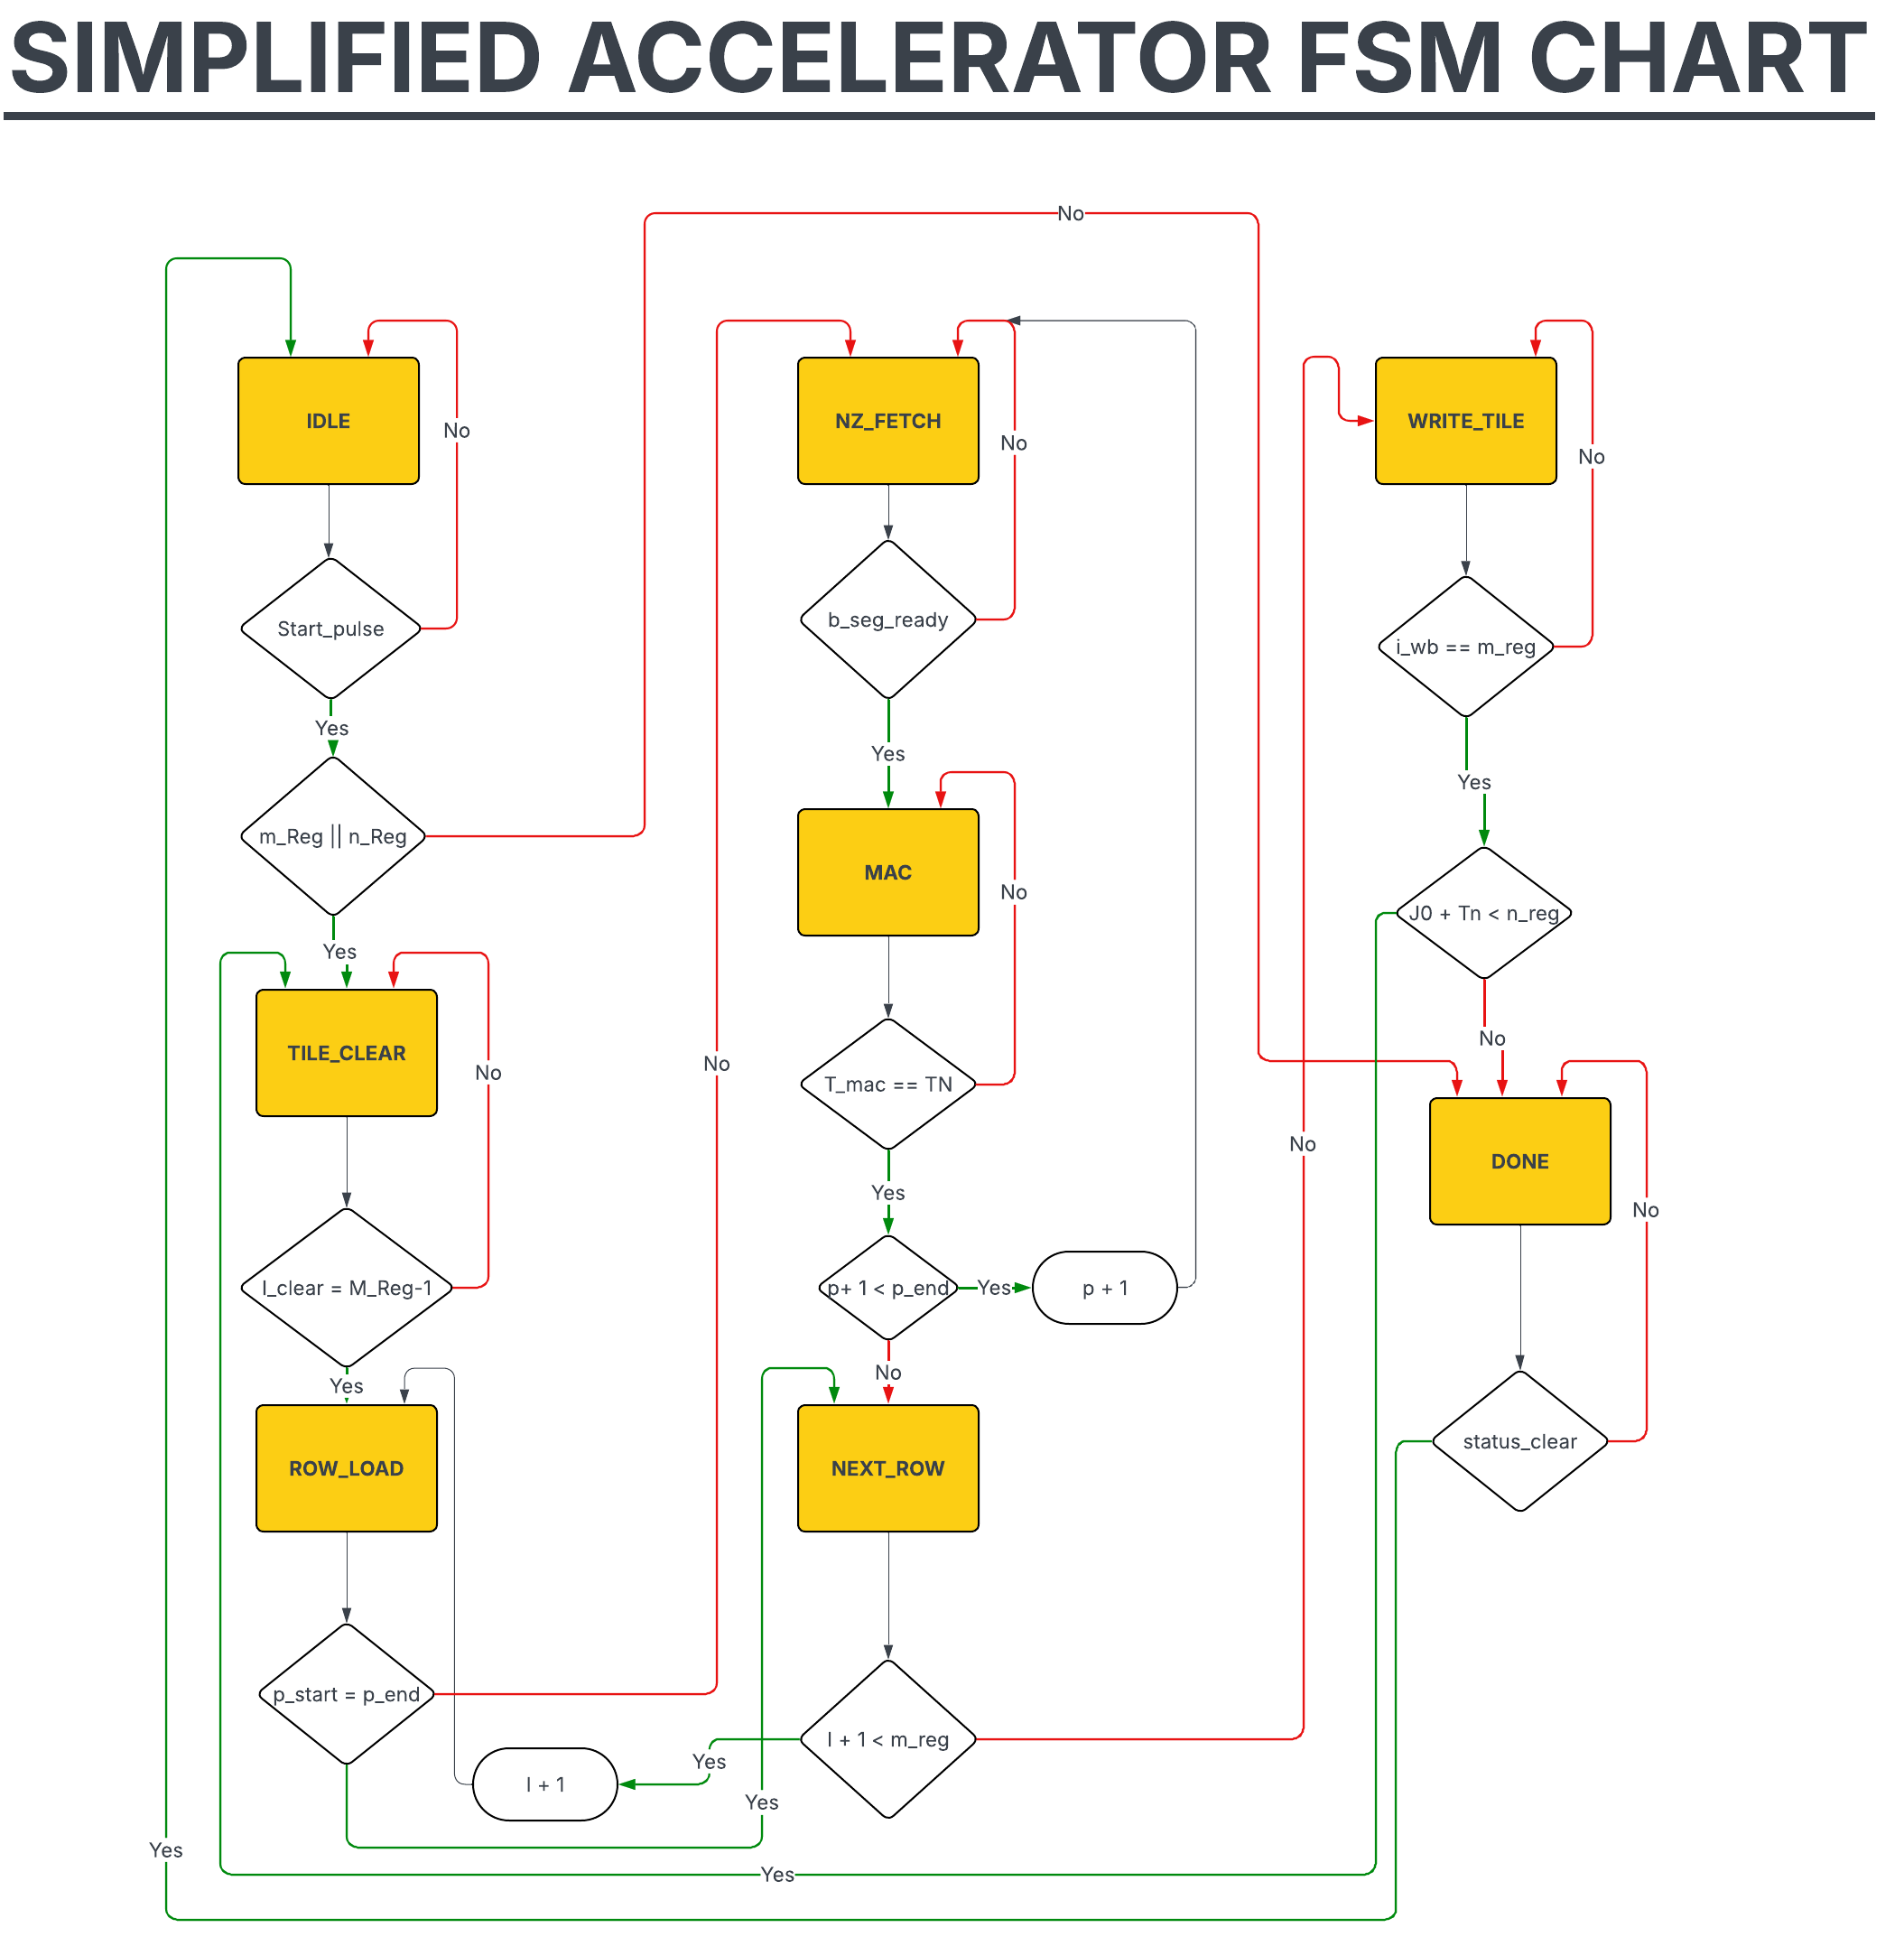
\includegraphics[width=\textwidth]{accel_fsm.png}
  \caption{Simplified accelerator finite state machine. Each major phase
           corresponds to one row in Table~\ref{tab:fsm-states}. Sub-phase
           transitions within \texttt{ROW\_LOAD} and \texttt{NZ\_FETCH}
           handle the one-cycle registered RAM output latency.}
  \label{fig:accel-fsm}
\end{figure}

For a matrix with $M$ rows, NNZ nonzeros, and dense width $N$ (processed
in $N/TN$ tile columns), the approximate cycle budget per tile column is
\[
  T_{\mathrm{tile}} \approx M_{\mathrm{max}} + M \cdot C_{\mathrm{row}}
  + \text{NNZ} \cdot (C_{\mathrm{nz}} + TN) + M \cdot TN \cdot C_{\mathrm{wb}},
\]
with $C_{\mathrm{row}} \approx 5$ cycles per row-bound load,
$C_{\mathrm{nz}} \approx 5$ cycles per nonzero fetch, and
$C_{\mathrm{wb}} \approx 1$ cycle per output writeback. At $TN = 8$ the
nonzero fetch and $B$-segment fill together contribute roughly
$5 + 8 = 13$ cycles per nonzero, and the reader will see directly how
shrinking the $TN$-dependent term is what the INT8 optimisation later
attacks.

\section{The Choice of Tile Width}
\label{sec:tn-choice}

The tile width $TN$ sets the degree of parallelism in the dense dimension,
and its selection is a balance between arithmetic throughput, register
array size, memory-access burden, and routing feasibility on the target
device. Table~\ref{tab:tn-tradeoffs} summarises the options. At $TN = 1$
the accelerator degenerates to a sequential MAC with no parallel benefit;
$TN = 4$ offers modest parallelism at the price of halving the reuse of
each fetched $B$ segment; $TN = 16$ or $TN = 32$ doubles or quadruples the
register array and the number of required DSP blocks, at which point both
routing congestion and timing closure become the limiting factor on a
Cyclone~V that already carries a CPU, BRAM, UART, and GPIO. A tile width
of eight maps cleanly onto eight DSP multiply--accumulate blocks, keeps
the 512-register C-tile within practical limits, and covers the smallest
benchmark width ($N = 8$) in a single tile column so no case in the suite
is penalised by tiling overhead. It was also the largest width that
consistently closed timing at 50\,MHz in preliminary synthesis, which
settled the choice for the final design.

\begin{table}[htbp]
  \centering
  \small
  \begin{tabular}{lccccp{3.8cm}}
  \toprule
  $TN$ & MAC lanes & Acc.\ registers & B-seg reads/NZ & DSP estimate & Notes \\
  \midrule
  1  & 1 & 64 & 1 & 1 &
    Minimal resources; no parallelism; effectively sequential. \\
  4  & 4 & 256 & 4 & 4 &
    Moderate parallelism; reduced register pressure. \\
  8  & 8 & 512 & 8 & 8 &
    \textbf{Design point.} Good balance; DSP-mappable; 512-reg array feasible. \\
  16 & 16 & 1024 & 16 & 16 &
    Doubles resources; increases routing congestion; timing harder to close. \\
  32 & 32 & 2048 & 32 & 32 &
    Likely infeasible on Cyclone~V; 2048-reg array exceeds practical limits. \\
  \bottomrule
  \end{tabular}
  \caption{Resource and performance implications of different tile widths
           $TN$. The accelerator implements $TN = 8$.}
  \label{tab:tn-tradeoffs}
\end{table}

\section{Algorithmic Decomposition: Row-Wise CSR Traversal}

The first and most consequential design decision was algorithmic: process
CSR rows serially and tile only the dense dimension. Alternatives such as
outer-product decomposition (as in OuterSPACE~\citep{outerspace2018}) or
intersection-based skipping (as in ExTensor~\citep{extensor2019}) can
deliver higher throughput in certain regimes, but they do so by introducing
index-merge networks, multi-port accumulation, and in some cases
content-addressable storage, none of which are feasible inside the SoC
budget of this project. Row-wise CSR traversal keeps the FSM tractable
enough to verify by hand, keeps the BRAM Port~B access pattern regular so
no bank conflicts arise, and keeps the C-tile writeback purely sequential
with no merge logic. The simplicity pays for itself in both correctness
confidence and timing-closure margin.

\section{Memory Optimisation: the B-Segment Bottleneck}

In the baseline configuration, filling \texttt{B\_Seg} for a single
nonzero requires $TN = 8$ consecutive 32-bit RAM reads. With the one-cycle
registered latency each fill therefore takes at least $TN + 1 = 9$ cycles,
and the subsequent MAC another cycle, so roughly ten cycles of useful work
accumulate per nonzero once the segment is in place. These reads dominate
the per-nonzero cost entirely, and any architectural improvement that
leaves them untouched is bounded in impact.

INT8 packing is the architectural lever that directly addresses the
bottleneck. With matrix $B$ stored as packed INT8 at four values per
32-bit word, two consecutive aligned 32-bit reads deliver all eight INT8
values required to fill a $TN = 8$ segment, and the hardware extracts the
individual bytes in a single combinatorial stage:
\begin{equation}
  \texttt{B\_Seg}[4k + b] = \mathrm{sign\_ext}_{8 \to 32}
  \!\left( \texttt{ram\_rdata}[8(b{+}1){-}1 : 8b] \right),
  \quad b \in \{0, 1, 2, 3\},
  \label{eq:byte-extract}
\end{equation}
where the selected byte is placed in the lower eight bits of a 32-bit
register and the upper 24 bits are filled with the sign of that byte.
The segment fill therefore drops from eight cycles to two, a $4\times$
reduction in the memory-bound component of the per-nonzero cycle budget,
with no additional pipeline stage and no change to accumulation precision.

\section{DSP-Oriented Parallel MAC Enhancement}

The second optimisation stage restructured the MAC array to increase the
fraction of DSP blocks utilised per cycle. On the Cyclone~V, each DSP
block implements an 18$\times$18-bit signed multiplier followed by a
dedicated accumulator register, but the synthesis tool maps RTL
multipliers onto these blocks only if the operand widths and
accumulation structure match the block's
configuration~\citep{intel_dsp_blocks}. In the baseline design the eight
MAC operations are described as generic 32-bit multipliers; depending on
register fan-out and routing pressure, Quartus may or may not pack them
into DSP blocks, and in practice some lanes were being inferred in ALM
logic.

The DSP MAC stage rewrites the multiply--accumulate explicitly in the
registered-feedback form that the tool recognises as DSP-friendly:
\[
  \texttt{C\_Tile}[i][c] \;\leftarrow\; \texttt{C\_Tile}[i][c] + a \cdot B[c],
\]
using 32-bit signed operands and a registered accumulator. With this
structure Quartus maps each of the eight MAC lanes independently onto a
dedicated DSP multiplier/accumulator block rather than inferring ALM-based
multiplier cascades, and the resulting design completes each MAC in one
clock cycle with less ALM logic and lower power dissipation. Across the
full 12-case benchmark sweep this stage reduced total accelerator offload
cycles from 427,299 to 324,568, a $1.32\times$ improvement. The modest
gain is itself the interesting result: it confirms that the baseline was
not limited by arithmetic execution, and that further attention has to be
paid to memory traffic if the speedup ceiling is to move.

\section{INT8 Mode at the Datapath Level}

When \texttt{CTRL.int8\_mode} is asserted, three specific aspects of the
datapath change. The CSR \texttt{values} array is now stored as packed
INT8, and the controller tracks the byte offset of the current nonzero
within its 32-bit word using a two-bit counter: for nonzero index $p$ the
byte offset is $b = p \bmod 4$ and the enclosing word lives at
\texttt{A\_VAL\_BASE} $+ \lfloor p/4 \rfloor \times 4$, from which the
same sign-extension circuit used for $B$-byte extraction
(Equation~\ref{eq:byte-extract}) recovers a full-precision 32-bit $a$
before multiplication. The $B$-segment fill is replaced with the two-read
path described in the previous section, filling all eight lanes of
\texttt{B\_Seg} in two cycles instead of eight. Accumulation itself is
unchanged: every entry of \texttt{C\_Tile} remains INT32 throughout
computation, sign extension before multiplication ensures that products
and partial sums are always full-precision signed integers, and the
writeback path and MMIO interface see no INT8-specific modification. The
net effect is a $4\times$ reduction in $B$-segment memory traffic with no
cost in accumulator precision, output format, or control complexity.

\section{Physical Design Tradeoffs}

Adding the C-tile register array, the $B$-segment buffer, and eight
DSP-mapped MAC lanes markedly increases the net fan-out between the
controller and the datapath. The \texttt{mac\_a} operand in particular
must be distributed to all eight multiplier inputs simultaneously, and on
the Cyclone~V a register with a fan-out of eight combined with several
other wide buses (the BRAM port, address lines, register-file data paths)
creates routing congestion that is not visible in RTL simulation. The
target frequency is 50\,MHz, giving a 20\,ns period, and although modern
FPGA synthesis comfortably reaches 100--200\,MHz with DSP-mapped
multipliers, the critical path in this design is not the multiplier
itself but the combinatorial logic that generates CSR addresses and feeds
eight parallel writes into the C-tile. One synthesis attempt during the
DSP MAC stage failed to close timing until routing-affinity settings were
adjusted, and the incident is the concrete source of the lesson recorded
in Chapter~\ref{ch:reflection} that parallelism in FPGA designs carries
costs beyond logic area.

Table~\ref{tab:design-evolution} summarises the three hardware stages in
terms of their key architectural attributes. The common thread across the
rows is that the MAC width, the accumulator precision, and the output
format remain fixed at eight lanes, INT32, and INT32 respectively; what
changes between stages is whether the MAC maps to DSP blocks explicitly
and how many RAM reads the $B$-segment fill demands. Those two changes
alone account for the full $2.87\times$ cycle reduction observed from
baseline to final INT8 build.

\begin{table}[htbp]
  \centering
  \small
  \begin{tabular}{lccc}
  \toprule
  Attribute & Baseline & DSP MAC & INT8 packed \\
  \midrule
  MAC lanes & 8 & 8 & 8 \\
  DSP mapping & Inferred & Explicit & Explicit \\
  B reads per NZ & 8 & 8 & 2 \\
  Operand bit-width & 32-bit & 32-bit & 8-bit (sign-ext to 32) \\
  Accumulator precision & INT32 & INT32 & INT32 \\
  Output format & INT32 & INT32 & INT32 \\
  Avg.\ speedup over PicoRV32 SW & $16.12\times$ & $20.87\times$ & $45.28\times$ \\
  \bottomrule
  \end{tabular}
  \caption{Architectural attributes and measured average speedup for each
           design stage across the 12-case benchmark suite.}
  \label{tab:design-evolution}
\end{table}

\chapter{Testing and Verification}
\label{ch:methodology}

\section{Verification Approach}

Verification was carried out at two complementary levels: RTL-level
simulation before synthesis, and hardware-level functional verification
on the physical FPGA after programming. This two-level approach is
standard in digital design practice~\citep{sze2017}. RTL simulation is
fast and exposes internal signals for inspection, but it cannot on its
own guarantee that timing closure and synthesis artefacts have not
introduced discrepancies between the simulated and deployed design;
hardware verification on the device closes that gap by exercising the
complete SoC end-to-end. A discrepancy at either level is sufficient to
fail a case, and every recorded cycle count in Chapter~\ref{ch:results}
was taken from a run that passed both.

Within the simulation level the testbench suite was deliberately
structured to combine the three verification styles used in
industry-grade digital flows: \emph{directed tests} for targeted
functional cases with hand-computed golden outputs, \emph{concurrent
SystemVerilog Assertions (SVA)} for always-on protocol and liveness
monitoring, and \emph{constrained-random stimulus with functional
coverage and a scoreboard} for exploring the input space beyond what
directed tests reach. Four SystemVerilog testbenches cover the design:
three unit testbenches under \texttt{tb/unit/} that target the
accelerator modules in isolation, and one integration testbench under
\texttt{tb/integ/} that exercises the full synthesisable SoC with
firmware loaded into a behavioural RAM model.

\subsection*{Unit Testbench: Datapath}

\texttt{accel\_datapath\_tb.sv} exercises the arithmetic datapath in
isolation. It contains six directed tests covering $B_\mathrm{Seg}$
load, MAC accumulation, C-tile clear, ReLU activation (positive, zero,
and negative inputs), signed MAC with negative operands, and a small
hand-computed $2 \times 2$ SpMM. On top of the directed tests the
testbench runs a constrained-random MAC-scoreboard test: a transaction
class with \texttt{rand} row and operand fields is randomised for each
of twenty MAC operations per iteration, and a parallel software model
of the C-tile is updated in lock-step with the DUT. At the end of each
iteration every accessible C-tile location is read back and compared
against the software reference; any mismatch is reported with the
exact $(\mathrm{row}, \mathrm{col})$ index and stops the test. Five
concurrent SVA properties run for the entire simulation: ReLU output
non-negativity when enabled, writeback pass-through when disabled,
one-hot datapath command exclusivity (clear, $B_\mathrm{Seg}$ write,
MAC, and writeback may not fire simultaneously), MAC row index in
range, and $B_\mathrm{Seg}$ index in range. A functional covergroup
records MAC row band (low / mid / high) crossed with operand sign
(positive / zero / negative) so that the random test has a visible
coverage metric for how much of the tile and operand space has been
exercised.

\subsection*{Unit Testbench: Control FSM}

\texttt{accel\_ctrl\_tb.sv} verifies control-path behaviour by
instantiating the control module together with a synchronous RAM model
with the same one-cycle read latency as the deployed BRAM, plus a
datapath stub. Six concurrent SVA properties monitor the FSM's external
contract for the whole simulation: single-port RAM exclusivity (read
and write strobes may not be simultaneously high), 32-bit address
alignment on every RAM access, quiescence of the RAM interface during
reset, mutual exclusion of the \texttt{BUSY} and \texttt{DONE} status
bits, FSM liveness (every \texttt{BUSY} rise must be followed by a
\texttt{BUSY} fall within one million cycles), and one-hot exclusivity
of the four datapath command outputs (\texttt{dp\_clear\_en},
\texttt{dp\_bseg\_we}, \texttt{dp\_mac\_en}, \texttt{dp\_wb\_en}). A
directed smoke test drives the FSM through a full start--busy--done
cycle and checks that the IRQ line asserts correctly when
\texttt{irq\_en} is set.

\subsection*{Unit Testbench: Accelerator Top}

\texttt{accel\_top\_tb.sv} is the most comprehensive unit testbench and
closes the loop across the MMIO front-end, the FSM, and the datapath.
Stimulus is structured into two classes following the
\emph{transaction / driver} pattern common in UVM-style flows but
implemented in plain SystemVerilog: \texttt{SpmmConfig} is a
transaction object with \texttt{rand} fields for $M$, $N$, $K$, and
\texttt{relu\_en} and an embedded covergroup over the relevant
combinations; \texttt{accel\_drivers} holds a virtual handle to the
DUT's MMIO interface and implements the \texttt{mmio\_read},
\texttt{mmio\_write}, and \texttt{wait\_done} protocol tasks so that
every test uses the same low-level interface sequencing. Five directed
tests verify MMIO register read/write coverage, the empty-matrix
($\mathrm{NNZ} = 0$) case, a hand-computed $2 \times 2 \times 8$ SpMM,
ReLU clamping of a negative partial sum, and the BUSY-mirror LED. A
sixth constrained-random test randomises twenty \texttt{SpmmConfig}
objects, runs each one through the full accelerator end-to-end, reads
back the output C matrix, and verifies element-by-element that it
matches the trivially computable all-zero golden output; after each
iteration the covergroup sampling is reported so that coverage
convergence is visible during simulation. Five concurrent SVA
properties guard invariants that must hold across every one of these
tests: single-port RAM exclusivity, RAM address alignment, reset
quiescence, \texttt{BUSY}/\texttt{DONE} status mutex, and top-level FSM
liveness. Different simulation seeds (\texttt{+SEED=N}) exercise
different configuration combinations; coverage-driven regressions
simply increase the seed count until every bin of the covergroup is
hit.

\subsection*{Integration Testbench: Full SoC}

\texttt{soc\_tb.sv} instantiates PicoRV32 together with the accelerator
and a 64\,KB behavioural RAM, loads the compiled firmware image into
the RAM via \texttt{\$readmemh}, releases reset, and lets the firmware
execute its full benchmark sequence until the CPU writes a sentinel
value to a pre-agreed result address. This closes the loop between the
software control flow described in Chapter~\ref{ch:firmware} and the
hardware being verified: any firmware change that breaks the MMIO
contract, any RTL change that breaks the firmware's assumed timing, or
any memory-map misconfiguration fails immediately in simulation before
being committed to a synthesis run. Five concurrent SVA properties
monitor the shared memory fabric: address-decode exclusivity between
the RAM region and the accelerator MMIO region, bounded CPU handshake
progress (\texttt{mem\_ready} must rise within 1024 cycles of
\texttt{mem\_valid}), accelerator RAM 32-bit address alignment,
accelerator RAM single-port exclusivity, and an IRQ-epoch guard that
ensures the accelerator's IRQ line can only rise after the accelerator
has actually been started.

\subsection*{Shared Infrastructure}

All four testbenches share the support files under \texttt{tb/common/}:
\texttt{clk\_reset.sv} provides the clock generator and reset task,
\texttt{tb\_pkg.sv} provides plusarg helpers
(\texttt{get\_plusarg\_int}, \texttt{has\_plusarg}) so every testbench
accepts \texttt{+SEED} and \texttt{+WAVES} uniformly,
\texttt{tb\_macros.svh} defines the line-number-tagged
\texttt{TB\_CHECK} and \texttt{TB\_FATAL} PASS/FAIL macros, and
\texttt{tb\_regmap.svh} centralises the MMIO register offsets and bit
positions so that they are declared once and \texttt{`include}d
everywhere, preventing silent drift between testbenches and RTL.

\subsection*{Hardware-Level Verification}

Hardware-level verification is embedded directly inside the firmware
benchmark harness described in Section~\ref{sec:data-prep}. For each
of the 12 cases and at each of the three accelerator stages, firmware
generates deterministic inputs from fixed seeds, computes the
quantised CPU reference using the \texttt{spmm\_cpu\_q8()} routine,
runs the accelerator on the same inputs, and invokes the
\texttt{array\_compare()} scoreboard to verify every element of the
accelerator output matches the software reference exactly. This
routine functions as a hardware-level golden-reference scoreboard: it
covers all $M \times N$ output elements on every run, and a single
incorrect element causes the case to fail and no performance number
to be recorded. The combination of RTL-level SVA monitoring,
randomised-scoreboard unit testbenches, and firmware-level
element-wise comparison on real silicon provides three independent
layers of functional checking before any cycle count is reported.

\section{Benchmark Suite Design}
\label{sec:bench-design}

The benchmark suite was designed to cover multiple independent axes of
performance variation so that the reasons behind speedup trends can be
identified analytically rather than anecdotally. Four axes were chosen:
matrix size ($M$, $K$), which governs the amortisation of fixed setup
overhead; dense output width $N$, which determines the number of tile
columns and the ratio of tile-management cycles to useful computation;
sparsity level, which sets NNZ and therefore the volume of useful
arithmetic per row traversal; and nonzero distribution pattern, which
exposes any sensitivity of the accelerator or CPU to the spatial layout
of the nonzeros. Table~\ref{tab:benchmark-inputs} lists all 12 cases
together with the axis of variation each one primarily addresses.

\begin{table}[htbp]
  \centering
  \scriptsize
  \setlength{\tabcolsep}{4pt}
  \begin{tabular}{llrp{2.6cm}p{5.4cm}}
  \toprule
  Test ID & $M \times K \times N$ & Sparsity & Pattern & Purpose \\
  \midrule
  T1  & $8 \times 8 \times 8$    & 75\% & Uniform &
    Small debug/sanity case; establishes minimum speedup in the suite. \\
  T2  & $16 \times 16 \times 8$  & 75\% & Uniform &
    Small size-scaling point; 4$\times$ more arithmetic than T1. \\
  T3  & $32 \times 32 \times 8$  & 75\% & Uniform &
    Medium size-scaling point. \\
  T4  & $64 \times 64 \times 8$  & 75\% & Uniform &
    Largest square case; maximum $M$ for the current $M_{\max} = 64$. \\
  T5  & $64 \times 64 \times 16$ & 75\% & Uniform &
    Tests effect of doubling dense width relative to T4. \\
  T6  & $64 \times 64 \times 32$ & 75\% & Uniform &
    Tests effect of quadrupling dense width; 4 tile columns. \\
  T7  & $32 \times 32 \times 32$ & 50\% & Uniform &
    Low sparsity (dense); more nonzeros per row than T8/T9. \\
  T8  & $32 \times 32 \times 32$ & 75\% & Uniform &
    Mid-sparsity reference; matches T10/T11 except pattern. \\
  T9  & $32 \times 32 \times 32$ & 90\% & Uniform &
    Very sparse; exposes overhead-to-arithmetic ratio. \\
  T10 & $32 \times 32 \times 32$ & 75\% & Row-skewed NNZ &
    Same NNZ as T8; row imbalance sensitivity. \\
  T11 & $32 \times 32 \times 32$ & 75\% & Clustered NNZ &
    Same NNZ as T8; block locality sensitivity. \\
  T12 & $64 \times 64 \times 32$ & 90\% & Uniform &
    Large sparse stress case; wide output and few nonzeros. \\
  \bottomrule
  \end{tabular}
  \caption{Complete benchmark input set used across all recorded
           evaluation stages.}
  \label{tab:benchmark-inputs}
\end{table}

\section{Cycle-Count Definitions and Speedup}

CPU cycle counts are measured around the timed software SpMM function
only. The measurement brackets the outer row loop, all CSR index reads
(\texttt{rowptr}, \texttt{colidx}), the inner dense-column MAC loop, and
all BRAM reads and writes to $B$ and $C$; matrix generation,
quantisation, and output-buffer clearing happen outside the bracket and
are deliberately excluded. Accelerator cycle counts are measured around
the complete \texttt{accel\_run\_spmm\_int8()} call and therefore include
the \texttt{clear\_done} write, the ten register writes of
\texttt{accel\_configure()} (roughly 20 cycles of overhead), the
\texttt{start} pulse, the complete hardware execution time, and the
polling loop that follows (about five cycles per iteration, typically no
more than ten iterations by the time \texttt{done} is observed). This
is an end-to-end offload latency from the CPU's perspective, which is
the correct metric for characterising user-visible benefit, but it is
explicitly not a measurement of pure datapath throughput.

Speedup is defined as
\[
  \text{Speedup} = \frac{T_{\mathrm{CPU}}}{T_{\mathrm{ACCEL}}},
\]
with both times measured in CPU clock cycles on the same 50\,MHz clock.
For the RISC-V comparisons $T_{\mathrm{CPU}}$ is the timed PicoRV32
software result (full INT32 for the baseline and DSP stages, INT8 for the
INT8 stage); for the Cortex-M0 comparison $T_{\mathrm{CPU}}$ is the
number of Cortex-M0 cycles computed from an equivalent instruction-count
model for the same benchmark case.

\section{Fairness, Limitations, and Threats to Validity}

The comparison is fair in several important respects. The CPU and
accelerator operate on the same benchmark inputs generated from the same
fixed seeds, they use the same shared on-chip RAM system at the same
50\,MHz clock, the software reference uses the M-extension \texttt{MUL}
instruction for its inner multiplies so that it is not artificially
slowed by software multiplication emulation, and the accelerator is
always validated against the software reference before its timing is
recorded. The Cortex-M0 comparison uses the same benchmark definitions
and the same accelerator cycle counts, with the CPU-side figures derived
from known Cortex-M0 instruction counts and the processor's published CPI
model (predominantly single-cycle instructions with 1--3 cycle load
latency). At the same time, the comparison differs in one important way:
the PicoRV32 software baseline runs on the very same in-order core that
controls the accelerator, with no cache, no speculation, and no SIMD. A
more aggressively optimised CPU implementation (one with
software-pipelined inner loops, block-reuse of $B$-rows, or explicit
prefetching) would narrow the gap. The goal of the baseline is
credibility and simplicity, not maximum CPU throughput.

Several limitations apply to all results presented in
Chapter~\ref{ch:results}. Each accelerator cycle count is a single
recorded value rather than a statistical distribution over multiple runs;
cycle counts for deterministic hardware are repeatable, but a
min/median/max summary would add an extra layer of confidence. The test
matrices are generated by a PRNG from fixed seeds rather than drawn from
real GNN or recommender-system datasets, so while they cover realistic
sparsity levels and pattern structures, performance on real workloads
may differ. All data lives in the 64\,KB on-chip BRAM; real SpMM
workloads typically span gigabytes and therefore incur DRAM latency,
and the results here reflect the best-case scenario of tightly coupled
on-chip memory. The accelerator cycle counts, as noted above, include
MMIO configuration and polling overhead, and for the smallest case (T1)
this overhead is a non-trivial fraction of the total. Finally, the
Quartus post-fit resource and timing reports were still being finalised
at the time of writing; the design has been verified to close timing at
50\,MHz, but the exact ALM, BRAM, and DSP counts across all three build
variants are pending.

These limitations define the scope of the claims that can be
responsibly made. The performance story (that INT8 packing delivers a
$2.18\times$ improvement over DSP MAC, which delivers a $1.32\times$
improvement over the baseline, and that memory bandwidth dominates the
cycle budget) is not undermined by any of them. But claims about
absolute performance at scale, DRAM bandwidth, or energy efficiency
would require a different experimental infrastructure than the one
developed here.

\chapter{Firmware and Software Control Flow}
\label{ch:firmware}

\section{Firmware Architecture and Memory Layout}

The bare-metal firmware is the software side of the hardware--software
co-design and is responsible for every aspect of the benchmark loop:
matrix generation, data preparation, accelerator configuration, timing
measurement, correctness checking, and result reporting. No operating
system is present; the firmware runs directly on PicoRV32 from address
\texttt{0x0000\_0000}. Control begins in \texttt{start.S}, a short
RISC-V assembly bootstrap that sets the stack pointer to the top of the
64\,KB RAM, clears the BSS section, and enters \texttt{main()}.
\texttt{main.c} itself defines the 12 test cases, iterates over them, and
for each case drives matrix generation, the software reference, the
accelerator launch, correctness comparison, and UART reporting. The
accelerator driver \texttt{spmm\_accel.c/.h} wraps the MMIO register
interface behind configuration, start, and polling functions, and a
handful of \texttt{memset}/\texttt{memcpy}/\texttt{memmove} stubs in
\texttt{libc\_stubs.c} cover the minimum set of C library calls required
for bare-metal operation. The linker script maps all sections
(\texttt{.text}, \texttt{.rodata}, \texttt{.data}, \texttt{.bss}) into the
same 64\,KB RAM, with the stack growing downward from the top.

Matrix buffers are allocated statically in the upper portion of the
address space, so that the CSR arrays, dense matrix $B$, and the output
matrices (\texttt{c\_accel} and \texttt{c\_cpu}) occupy contiguous regions
below the stack. The largest benchmark (T6: $64 \times 64 \times 32$,
75\% sparsity, NNZ~$\approx 1024$) consumes roughly
\[
  \underbrace{65 \times 4}_{\texttt{rowptr}} +
  \underbrace{1024 \times 4}_{\texttt{colidx}} +
  \underbrace{1024 \times 4}_{\texttt{values}} +
  \underbrace{64 \times 32 \times 4}_{B} +
  \underbrace{64 \times 32 \times 4}_{C} \approx 29\,\text{KB}
\]
of matrix data, leaving comfortable headroom in the 64\,KB budget for
firmware code and stack.

\section{Runtime Data Preparation}
\label{sec:data-prep}

Dense matrix $B$ is generated from a linear congruential PRNG seeded by
the benchmark case's \texttt{seed} field, with each entry sampled as a
signed integer in the range $[-127, 127]$ (directly usable as INT32 in
the full-precision path, and as the pre-quantisation domain for the INT8
path). Fixing the seed makes $B$ deterministic across runs and across
firmware revisions, which is what makes cycle-count regression comparison
across the three optimisation stages meaningful in the first place.

Sparse matrix $A$ is generated in three phases. Nonzero positions are
placed first, according to the pattern selected by the benchmark case.
For a uniform pattern, each row $i$ receives a target count
$n_i = \lfloor K(1 - s/100) \rfloor$ of nonzeros at column indices
sampled without replacement from the PRNG; for a row-skewed pattern,
roughly 30\% of the rows receive a disproportionate share of the total
NNZ budget, simulating the hub-node behaviour characteristic of social
graphs; and for a clustered pattern, nonzeros are biased toward
rectangular blocks within the matrix, mimicking the blocked sparsity seen
in some finite-element problems. Each placed nonzero then receives a
random signed value in $[-127, 127]$. Finally, the CSR representation is
constructed: column indices within each row are sorted in ascending order
(required for determinism and for correct comparison against the CPU
reference), \texttt{rowptr} is produced by a prefix sum of per-row
nonzero counts, and the sorted indices and values are written to
\texttt{colidx} and \texttt{values}. Sorting column indices also makes
the CSR representation canonical across runs, which simplifies debugging
whenever an accelerator output needs to be compared by hand against the
expected reference.

\section{Software Baseline}

The software reference is deliberately written in the simplest possible
form. The full-precision inner structure is:
\begin{verbatim}
for (row = 0; row < M; row++) {
    for (p = rowptr[row]; p < rowptr[row+1]; p++) {
        col = colidx[p];
        a   = values[p];
        for (n = 0; n < N; n++)
            C[row*N + n] += a * B[col*N + n];
    }
}
\end{verbatim}
\noindent\textbf{Listing~\ref{lst:spmm-cpu}}: PicoRV32 software SpMM
(full precision).
\label{lst:spmm-cpu}

Only the M-extension \texttt{MUL} instruction is used for the inner
multiply. There is no SIMD, no loop unrolling, and no software
prefetching. This simplicity is intentional: the point of the baseline is
not to measure the fastest CPU implementation possible but to give a
credible, readable software reference against which the accelerator's
structural advantage can be isolated. The INT8 CPU reference
(\texttt{spmm\_cpu\_q8}) follows the same structure but operates on
signed 8-bit operands with INT32 accumulation, and it is the version used
for correctness comparison against the INT8 accelerator output.

\section{INT8 Quantisation and Packing}
\label{sec:quant-flow}

Before an INT8 accelerator run, firmware applies symmetric runtime
quantisation separately to the CSR values array and to matrix $B$.
For a vector $\mathbf{v}$ of length $L$, the procedure computes
$v_{\max} = \max_i |v_i|$, sets scale $s = v_{\max}/127$, and quantises
each element as $q_i = \mathrm{clip}(\mathrm{round}(v_i/s), -127, 127)$.
The edge case $v_{\max} = 0$ is handled by setting all quantised values
to zero and $s = 1$. This matches Equation~\ref{eq:quant} from
Section~2.6. The scale factor is computed and then discarded at
quantisation time: since the correctness check compares accelerator
output against the \emph{quantised} CPU reference (which accumulates the
same signed INT8 values), there is no need to store $s$, and keeping the
path scale-free simplifies both the accumulator logic and the verification.

After quantisation, four consecutive INT8 values are packed into a single
32-bit word in little-endian byte order:
\begin{verbatim}
for (i = 0; i < len; i += 4) {
    word = ((uint32_t)(uint8_t)q[i+0])        |
           ((uint32_t)(uint8_t)q[i+1] << 8)   |
           ((uint32_t)(uint8_t)q[i+2] << 16)  |
           ((uint32_t)(uint8_t)q[i+3] << 24);
    dst[i/4] = word;
}
\end{verbatim}

Matrix $B$ is packed row by row, so a single 32-bit RAM read on the
hardware side delivers four aligned INT8 values and directly populates
four lanes of the $B$-segment buffer after sign extension, exactly as
described in Section~\ref{sec:fsm}.

\section{Accelerator Launch and Timing}

The accelerator driver exposes \texttt{accel\_configure()} for writing
dimension and base-address registers, \texttt{accel\_start\_mode()} for
issuing the control write with the \texttt{start} pulse and the
\texttt{relu\_en}/\texttt{int8\_mode} bits, and \texttt{accel\_wait\_done()}
for polling \texttt{STATUS.done}. \texttt{accel\_run\_spmm\_int8()} wraps
these into the canonical launch sequence used on every benchmark case.
Firmware first writes \texttt{clear\_done} to reset any prior completion
state, calls \texttt{accel\_configure()} to set dimensions and base
addresses, captures the pre-launch cycle count $t_0$, issues the
\texttt{start}-mode write, polls \texttt{STATUS.done} in a tight loop,
captures the post-completion cycle count $t_1$, writes \texttt{clear\_done}
once more to reset for the next run, and reports $t_1 - t_0$ as the
accelerator cycle count. The reported figure therefore includes register
write overhead, the full hardware execution time, and the polling loop
delay, and is explicitly an end-to-end offload latency rather than a pure
datapath throughput measurement.

Timing itself relies on the PicoRV32 \texttt{rdcycle} CSR, which returns
the lower 32 bits of a monotonically increasing hardware cycle counter
clocked at 50\,MHz. The read is wrapped in a short inline assembly stub:
\begin{verbatim}
static inline uint32_t read_cycles(void) {
    uint32_t cyc;
    asm volatile("rdcycle %0" : "=r"(cyc));
    return cyc;
}
\end{verbatim}

The 32-bit counter wraps at $2^{32}$ cycles, which at 50\,MHz is
approximately 85 seconds. The largest benchmark in the suite completes
in fewer than two million cycles, so wrap-around is not a concern and no
32-to-64-bit extension is required in firmware.

\section{Reporting and Correctness Verification}

Results are output as CSV-formatted lines over the on-chip UART at
115200\,baud (50\,MHz / 434 cycles per bit), with each line containing
the test ID, the dimensions $M$, $K$, $N$, the sparsity percentage and
pattern, the NNZ count, the CPU and accelerator cycle counts, the derived
speedup, and a PASS/FAIL verdict. A simplified summary is also driven
onto the DE1-SoC's six seven-segment displays (the upper pair shows
CPU cycles scaled by 64, the middle pair shows raw accelerator cycles,
and the lower pair shows integer speedup), so that a running benchmark
can be read at a glance without a host terminal. The LED output mirrors
the busy/done signals, so visually the board is lit during accelerator
execution and cleared the moment computation completes.

Correctness verification is embedded directly in the benchmark loop:
after each accelerator run, firmware performs an element-by-element
comparison between \texttt{c\_accel} and the INT8 CPU reference
\texttt{c\_cpu}:
\begin{verbatim}
for (i = 0; i < M*N; i++) {
    if (c_accel[i] != c_cpu[i]) {
        pass = 0; break;
    }
}
\end{verbatim}
The full-precision CPU result is also computed in parallel but untimed,
and serves as a sanity reference against which quantisation error can be
inspected if needed. Because both the CPU and the accelerator apply the
same symmetric INT8 quantisation to the same input data and accumulate
identical INT32 partial sums, their outputs must match exactly, and any
discrepancy flags a hardware bug rather than a numerical artefact. All
12 cases reported PASS across all three accelerator stages on hardware.

\chapter{Reflection}
\label{ch:reflection}

\section{What Worked Well}

Structuring development as a sequence of discrete, measurable optimisation
stages (baseline, DSP MAC, and INT8 packing) was the single most valuable
decision in the project. A working baseline was established and verified on
hardware before any optimisation was attempted, and each subsequent stage
changed exactly one aspect of the design: arithmetic parallelism first, then
memory traffic. This made it possible to attribute each measured improvement
to a specific architectural change, to detect regressions immediately, and to
build the evidence-based narrative used throughout Chapter~\ref{ch:results}.

The deterministic benchmark harness was equally important. Generating all
test inputs from fixed seeds at runtime, and computing golden outputs on the
same PicoRV32 host, removed the need for off-chip reference data and ensured
that the same matrices were used across all three hardware stages. Any
functional discrepancy introduced by a hardware or software change would have
been caught by the element-by-element comparison on the next rebuild.

The roofline analysis in Chapter~\ref{ch:motivation} correctly predicted before
implementation that memory traffic, not arithmetic, would be the dominant
bottleneck. The measured $1.32\times$ gain from DSP-based MAC compared to the
$2.18\times$ gain from INT8 packing confirmed this diagnosis quantitatively. A
design effort that had focused purely on widening the MAC array would have
yielded diminishing returns; addressing the memory bottleneck directly produced
the largest single performance step.

\section{What Went Wrong and What Was Learned}

The most time-consuming debugging episode involved a stale
\texttt{firmware.mif} file. The FPGA synthesis flow uses this memory
initialisation file to preload on-chip RAM with the compiled firmware image.
When the file was not regenerated after a firmware change, the board continued
to run the previous image while the expected code had in fact been rebuilt.
Diagnosing this required noticing that on-board UART output did not match the
current source, which was non-trivial when the visible output is only a few bytes. The
lesson is that FPGA flows combining independently compiled software and
hardware artefacts require explicit dependency management in the build system;
a Makefile rule that re-triggers synthesis on \texttt{firmware.mif} changes
would have prevented the issue entirely.

A second lesson came from increasing routing pressure as parallel logic was
added. Quartus reported higher congestion around the C-tile register array
and the wide MAC buses, and timing closure failed after the INT8 packing
datapath was introduced until the fitter was switched from the default
balanced optimisation mode to performance-oriented optimisation.
Parallelism in FPGA designs carries costs beyond logic area: routing,
placement, and timing closure are interdependent, and a design that fits
comfortably in ALMs can still fail to close timing if the wiring density in
a local region exceeds the device's capacity. This tension does not appear
in RTL simulation and cannot be resolved by functional correctness alone.

\section{Project Management}

The project ran across two semesters. Semester~1 covered the literature
review, the design and planning phases, RTL development and integration,
and the initial FPGA deployment. Semester~2 covered the two remaining
optimisation stages (DSP-oriented MAC and INT8 quantisation), the hardware
benchmarking campaign, and report writing. The Gantt charts in
Appendix~\ref{app:gantt} record both the original plan and the way the
work actually unfolded.

Semester~1 schedule pressure arose almost entirely from the implementation
and integration phases, which ultimately ran roughly two weeks longer than
the planned allocation, as noted in Appendix~\ref{app:gantt}. Three
factors contributed. First, RTL verification exposed a combination of
syntax errors and functional defects in the early testbenches, each of
which required targeted debugging before the unit suites would pass.
Second, the SoC was originally specified with an interrupt-driven
completion path from the accelerator to the CPU, but the unforeseen
complexity of integrating interrupt handling with the PicoRV32 exception
model led to the mechanism being descoped in favour of a simple polling
loop on the status register. Third, the plan allocated only a four-day
slack window (22--25 December) for unforeseen errors, which was consumed
almost immediately once the integration problems began to appear and
proved far too short for a project of this scale.

Semester~2 pressure originated mainly from the benchmarking phase. The
UART peripheral bundled with the PicoRV32 reference design did not
support the cycle-accurate timing readouts required by the measurement
methodology in Chapter~\ref{ch:methodology}, which blocked progress on
the benchmark harness until a replacement was identified. Adopting the
open-source \texttt{simpleuart} core resolved this and removed the
largest single source of benchmarking delay. The stale firmware image
bug discussed in the preceding section compounded the pressure by
masquerading as functional failure for several days before the root
cause was understood. Finally, after the INT8 packing datapath was
added, Quartus routing failed to close timing under the default balanced
optimisation mode; switching the fitter to performance-oriented
optimisation closed timing but added roughly twenty minutes to every
full synthesis run, which measurably lengthened the remaining debug
iterations. Preserving a fully working, deployable design at the end of
every stage, rather than accumulating partially integrated features,
was the practice that kept the overall schedule recoverable despite
these setbacks.

The overarching lesson is that hardware project timelines are dominated
by integration and debug rather than initial design. Treating build-flow
discipline (artefact management, synthesis scripts, timing closure) as
first-class engineering work from the outset, rather than as polish at
the end, would have eliminated most of the schedule pressure experienced
in the second half of the project.

% !TEX root = ../main.tex
\chapter{Conclusion}
\label{ch:conclusion}

\section{Summary of Achievements}

This project set out to design, implement, and evaluate a RISC-V-attached
hardware accelerator for CSR sparse matrix--dense matrix multiplication on the
Terasic DE1-SoC, and to demonstrate a measurable speedup over software while
remaining reproducible at the register-transfer level. That aim was met. A
complete PicoRV32 SoC with a working SpMM accelerator, 64\,KB shared
dual-port BRAM, MMIO interface, and UART reporting was synthesised and
deployed; three recorded optimisation stages (baseline, DSP-enhanced, and
INT8 packed) were each verified for correctness on hardware; and a 12-case
benchmark harness with deterministic matrix generation, cycle-accurate timing,
and element-by-element correctness checking was developed to evaluate them.

The final INT8-packed implementation achieves a peak speedup of
$\mathbf{56.80\times}$ over the quantised PicoRV32 software reference and
$\mathbf{11.92\times}$ over an ARM Cortex-M0 baseline running the same
algorithm, with an average of $45.28\times$ and $9.79\times$ respectively
across the 12-case suite. All 12 cases passed correctness checks at every
stage.

\section{Significance}

The significance of this work lies not in the absolute numbers compared to
large research accelerators, but in what the staged measurement reveals about
the workload. The $1.32\times$ gain from DSP-based MAC versus the
$2.18\times$ gain from INT8 packing experimentally confirms that the dominant
bottleneck in CSR SpMM on a memory-bandwidth-constrained embedded FPGA is
operand fetch traffic, not arithmetic execution. This is a useful result
beyond the specific artefact: it indicates that similar embedded accelerators
should prioritise format-level and precision-level optimisations over wider
MAC arrays. The project also demonstrates that a fully integrated, firmware-
driven hardware benchmark harness is a practical alternative to external
simulation infrastructure for small-scale accelerator evaluation, and that a
useful SpMM accelerator fits comfortably within the resource budget of a
Cyclone~V device.

\section{Future Work}

The most impactful extensions to the current design would be:

\begin{enumerate}
  \item \textbf{Wider tile width.} INT8 packing reduces the per-nonzero fetch
        cost enough that widening from $TN = 8$ to $TN = 16$ or $TN = 32$ is
        now attractive. Doubling the tile width costs an additional two
        32-bit reads per nonzero but delivers $2\times$ the MAC throughput
        per nonzero, and should push the speedup ceiling further.

  \item \textbf{Ping-pong $B$-segment prefetch.} Double-buffering the
        $B$-segment allows the next segment to be fetched while the current
        MAC operation completes, overlapping memory latency with arithmetic
        and removing it from the critical path.

  \item \textbf{External memory interface.} Extending the design to address
        off-chip SDRAM or HPS DRAM through the DE1-SoC's HPS bridge would
        permit realistically sized GNN and recommender-system matrices to
        be benchmarked, at which point off-chip bandwidth becomes the
        dominant term and different optimisations become relevant.

  \item \textbf{Interrupt-driven completion.} Replacing the polling loop
        with a RISC-V interrupt handler would free the CPU during
        accelerator execution, enabling pipelined benchmark preparation or
        post-processing of the previous result.

  \item \textbf{Power and energy characterisation.} Instrumenting the
        DE1-SoC rails or using Quartus Power Analyser with simulation-derived
        toggle files would add energy efficiency to the evaluation, which is
        the metric that matters most in the embedded and edge contexts for
        which this class of accelerator is targeted.
\end{enumerate}

\section{Closing Remarks}

This project has delivered a complete, measured, and reproducible RISC-V
FPGA-attached SpMM accelerator that achieves a peak speedup of $56.80\times$
on hardware through three progressively optimised designs. The work confirms
that even without exotic hardware resources or advanced scheduling, careful
alignment of the memory format, datapath structure, and quantisation strategy
with the actual bottleneck of the workload produces large, predictable, and
experimentally confirmed performance gains.


% ------------------------------------------------------------
% Resolve citation numbers by reading the bibliography into a
% discarded box. \bibitem still writes \bibcite to the .aux file
% as a side effect, so \cite{...} expands to the correct number,
% but nothing visible is emitted and no pages are added. This
% keeps the shortened document's page numbering aligned with the
% full archive copy.
% ------------------------------------------------------------
\makeatletter
\let\bibsection\relax
\renewenvironment{thebibliography}[1]{%
  \setbox\@tempboxa=\vbox\bgroup
    \list{\@biblabel{\the\c@NAT@ctr}}{%
      \labelsep=0pt\labelwidth=0pt\leftmargin=0pt\itemindent=0pt%
      \@bibsetup{#1}\global\c@NAT@ctr\z@%
    }%
    \sloppy\clubpenalty=4000\widowpenalty=4000%
    \sfcode`\.=\@m
}{%
    \def\@noitemerr{\@latex@warning{Empty bibliography}}%
    \endlist
  \egroup
}
\makeatother
\bibliographystyle{unsrtnat}
\bibliography{bib/ECS}

\end{document}
